\chapter{Anexo}
\label{cap:anexo}

\begin{figure}[ht!]
  \centering
  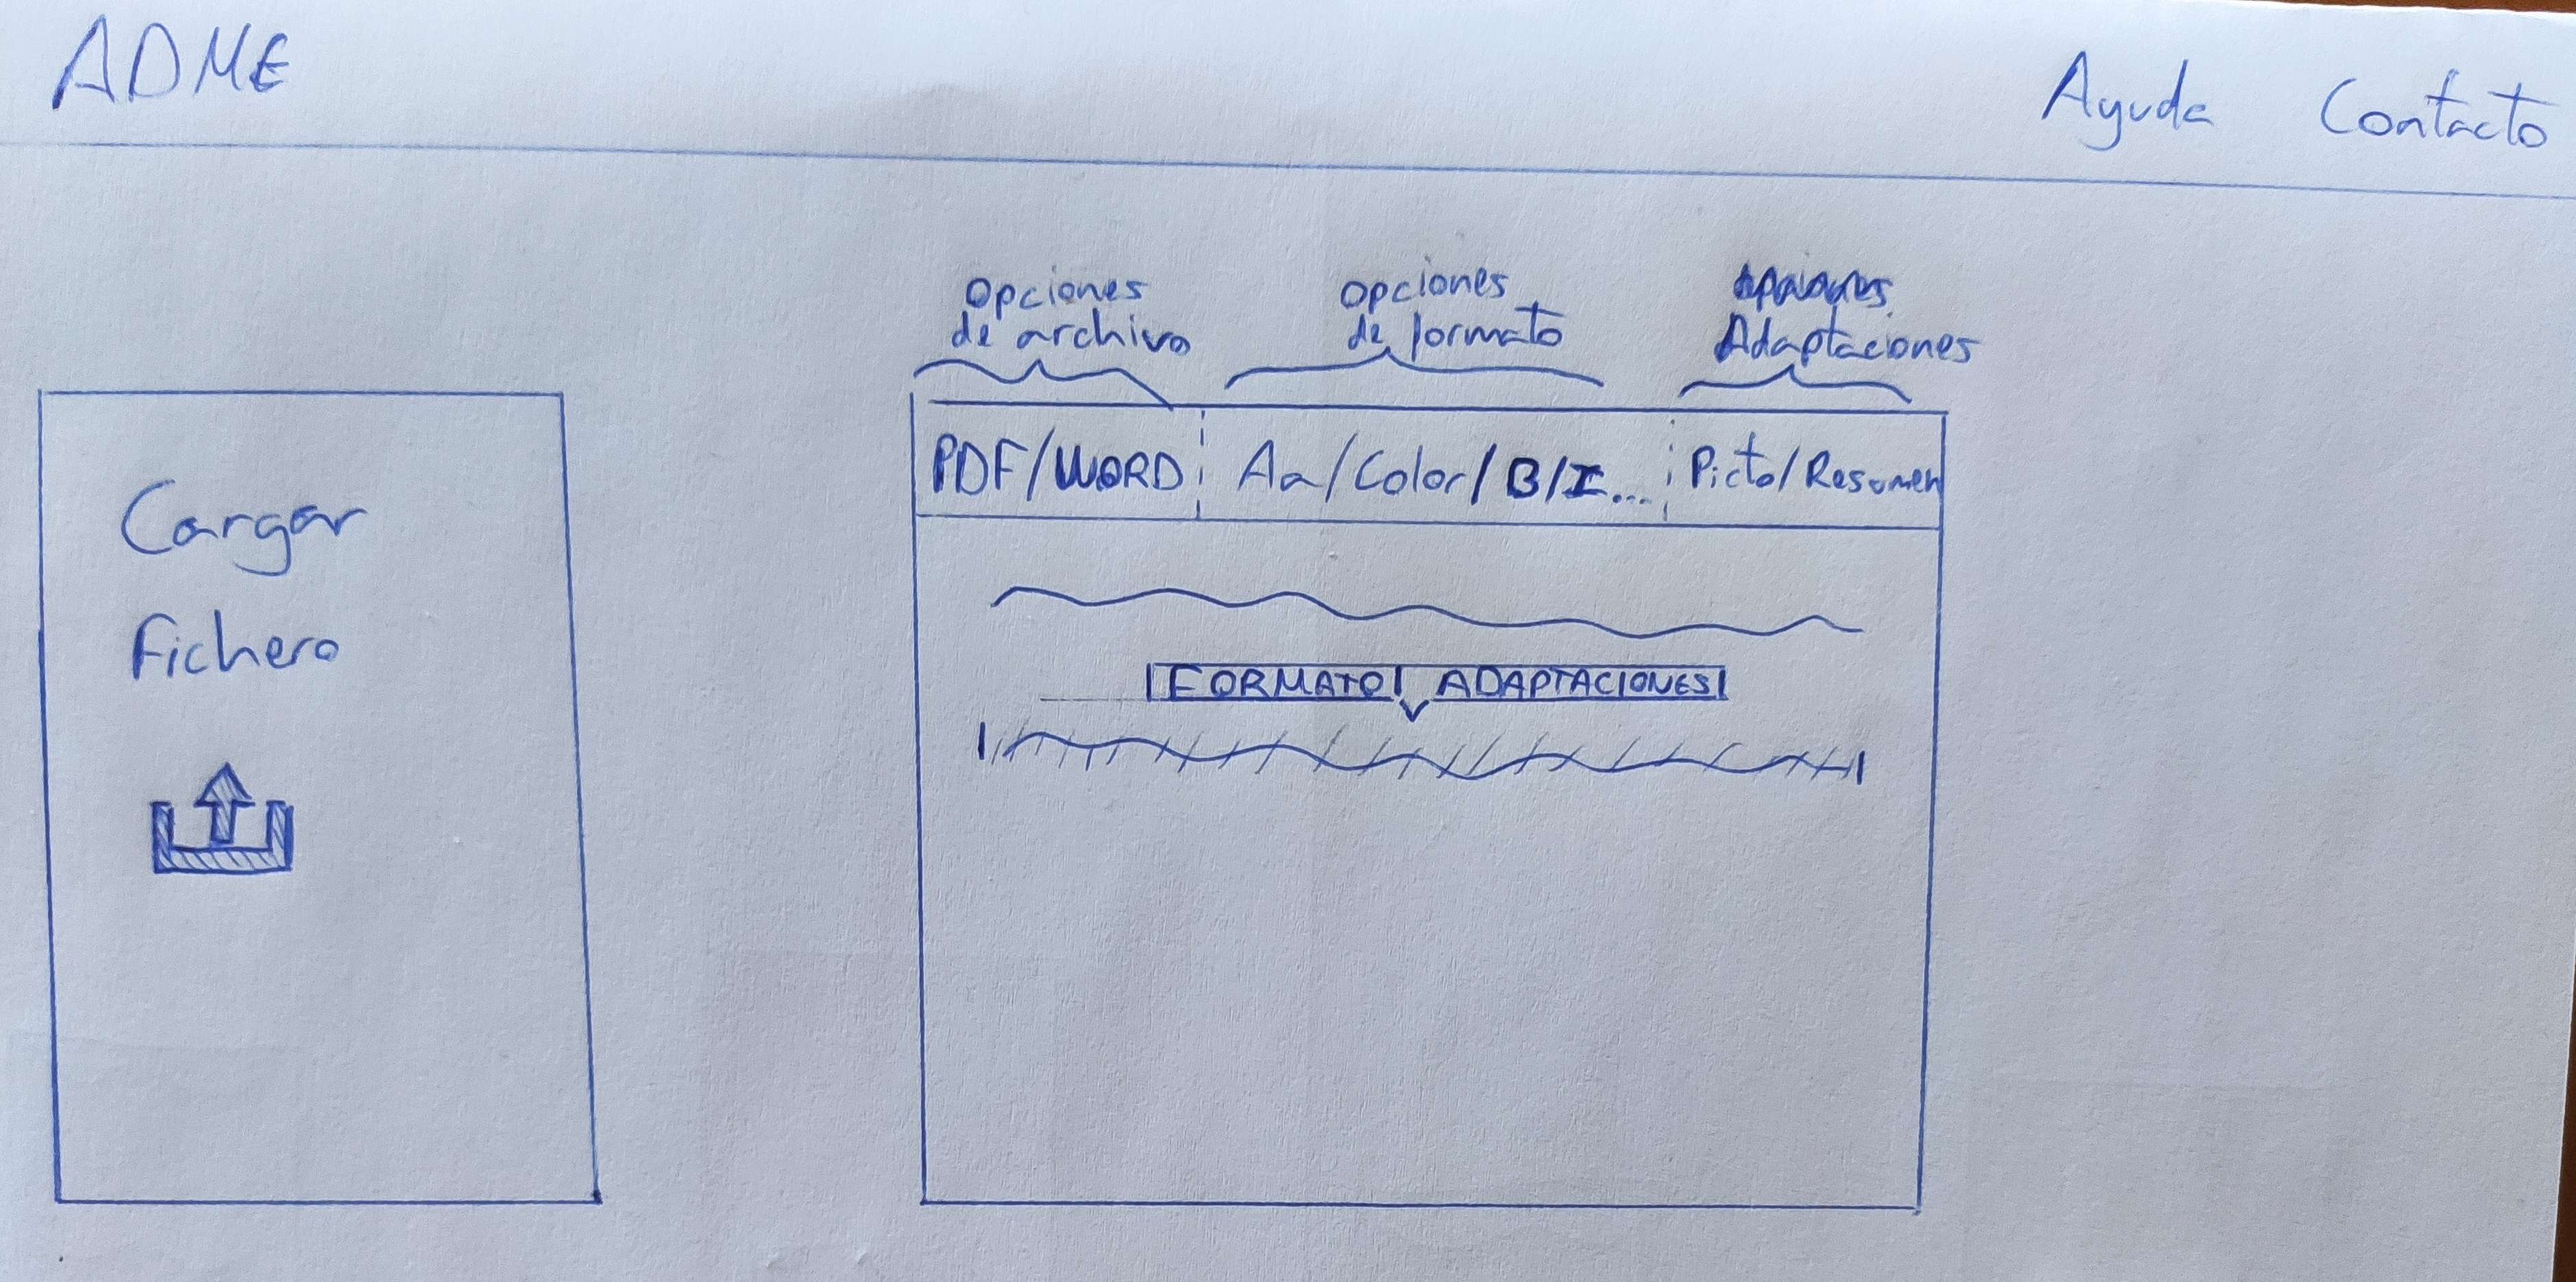
\includegraphics[width=10cm]{Diseño/Alvaro/Alvaro01.jpg}
  \caption{Diseño pantalla de inicio de Álvaro sin PDF.}
  \label{fig:disenyoAlvaro01}
\end{figure}

\begin{figure}[ht!]
  \centering
  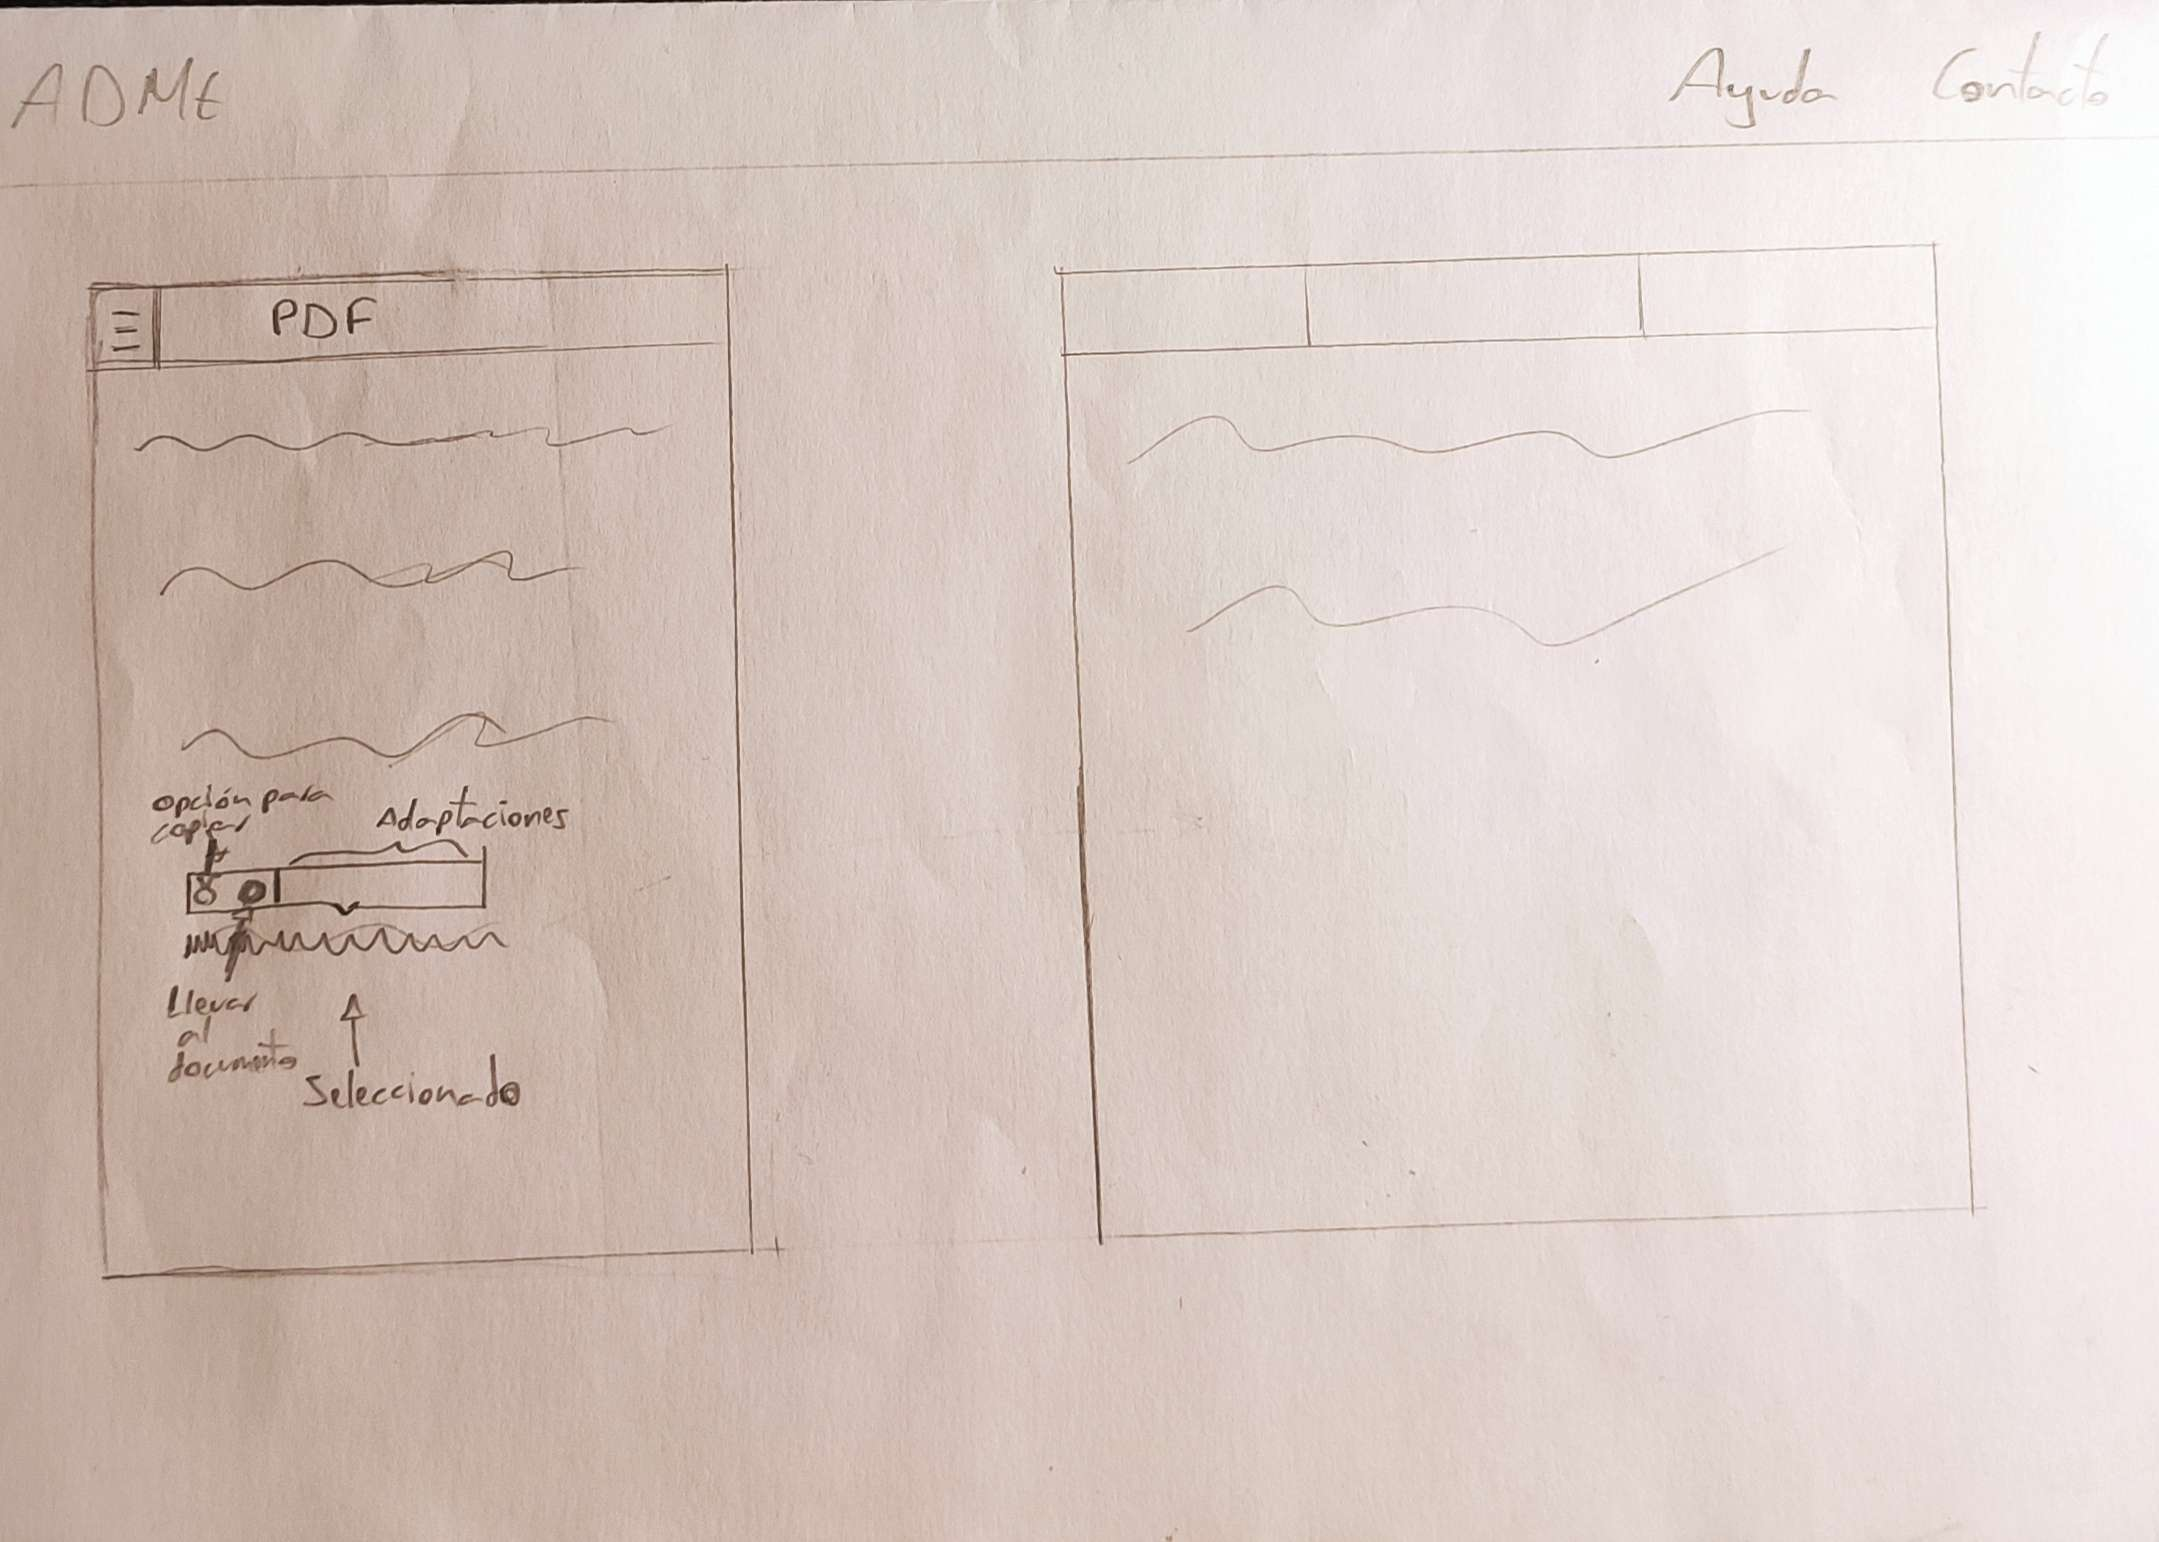
\includegraphics[width=10cm]{Diseño/Alvaro/Alvaro02.jpg}
  \caption{Diseño pantalla de inicio de Álvaro con PDF.}
  \label{fig:disenyoAlvaro02}
\end{figure}

\begin{figure}[ht!]
  \centering
  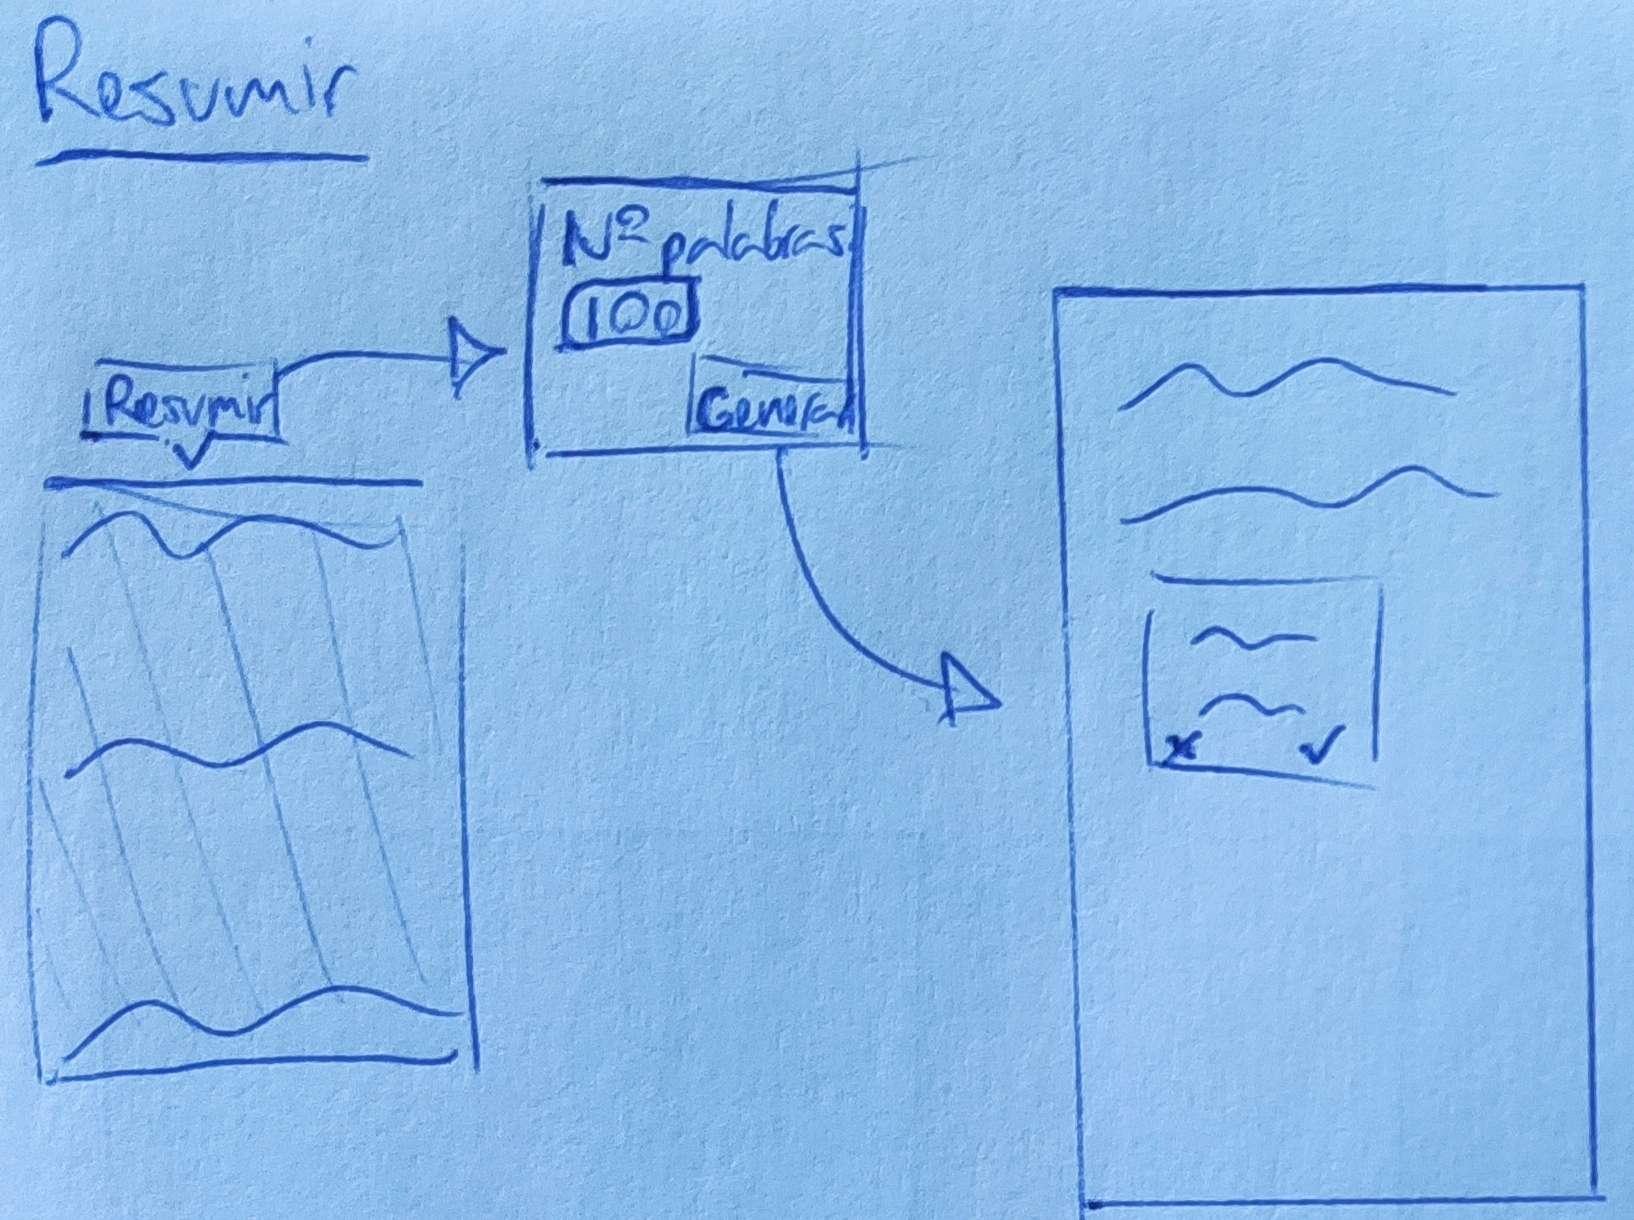
\includegraphics[width=10cm]{Diseño/Alvaro/Alvaro03.jpg}
  \caption{Diseño generar resumen de Álvaro.}
  \label{fig:disenyoAlvaro03}
\end{figure}

\begin{figure}[ht!]
  \centering
  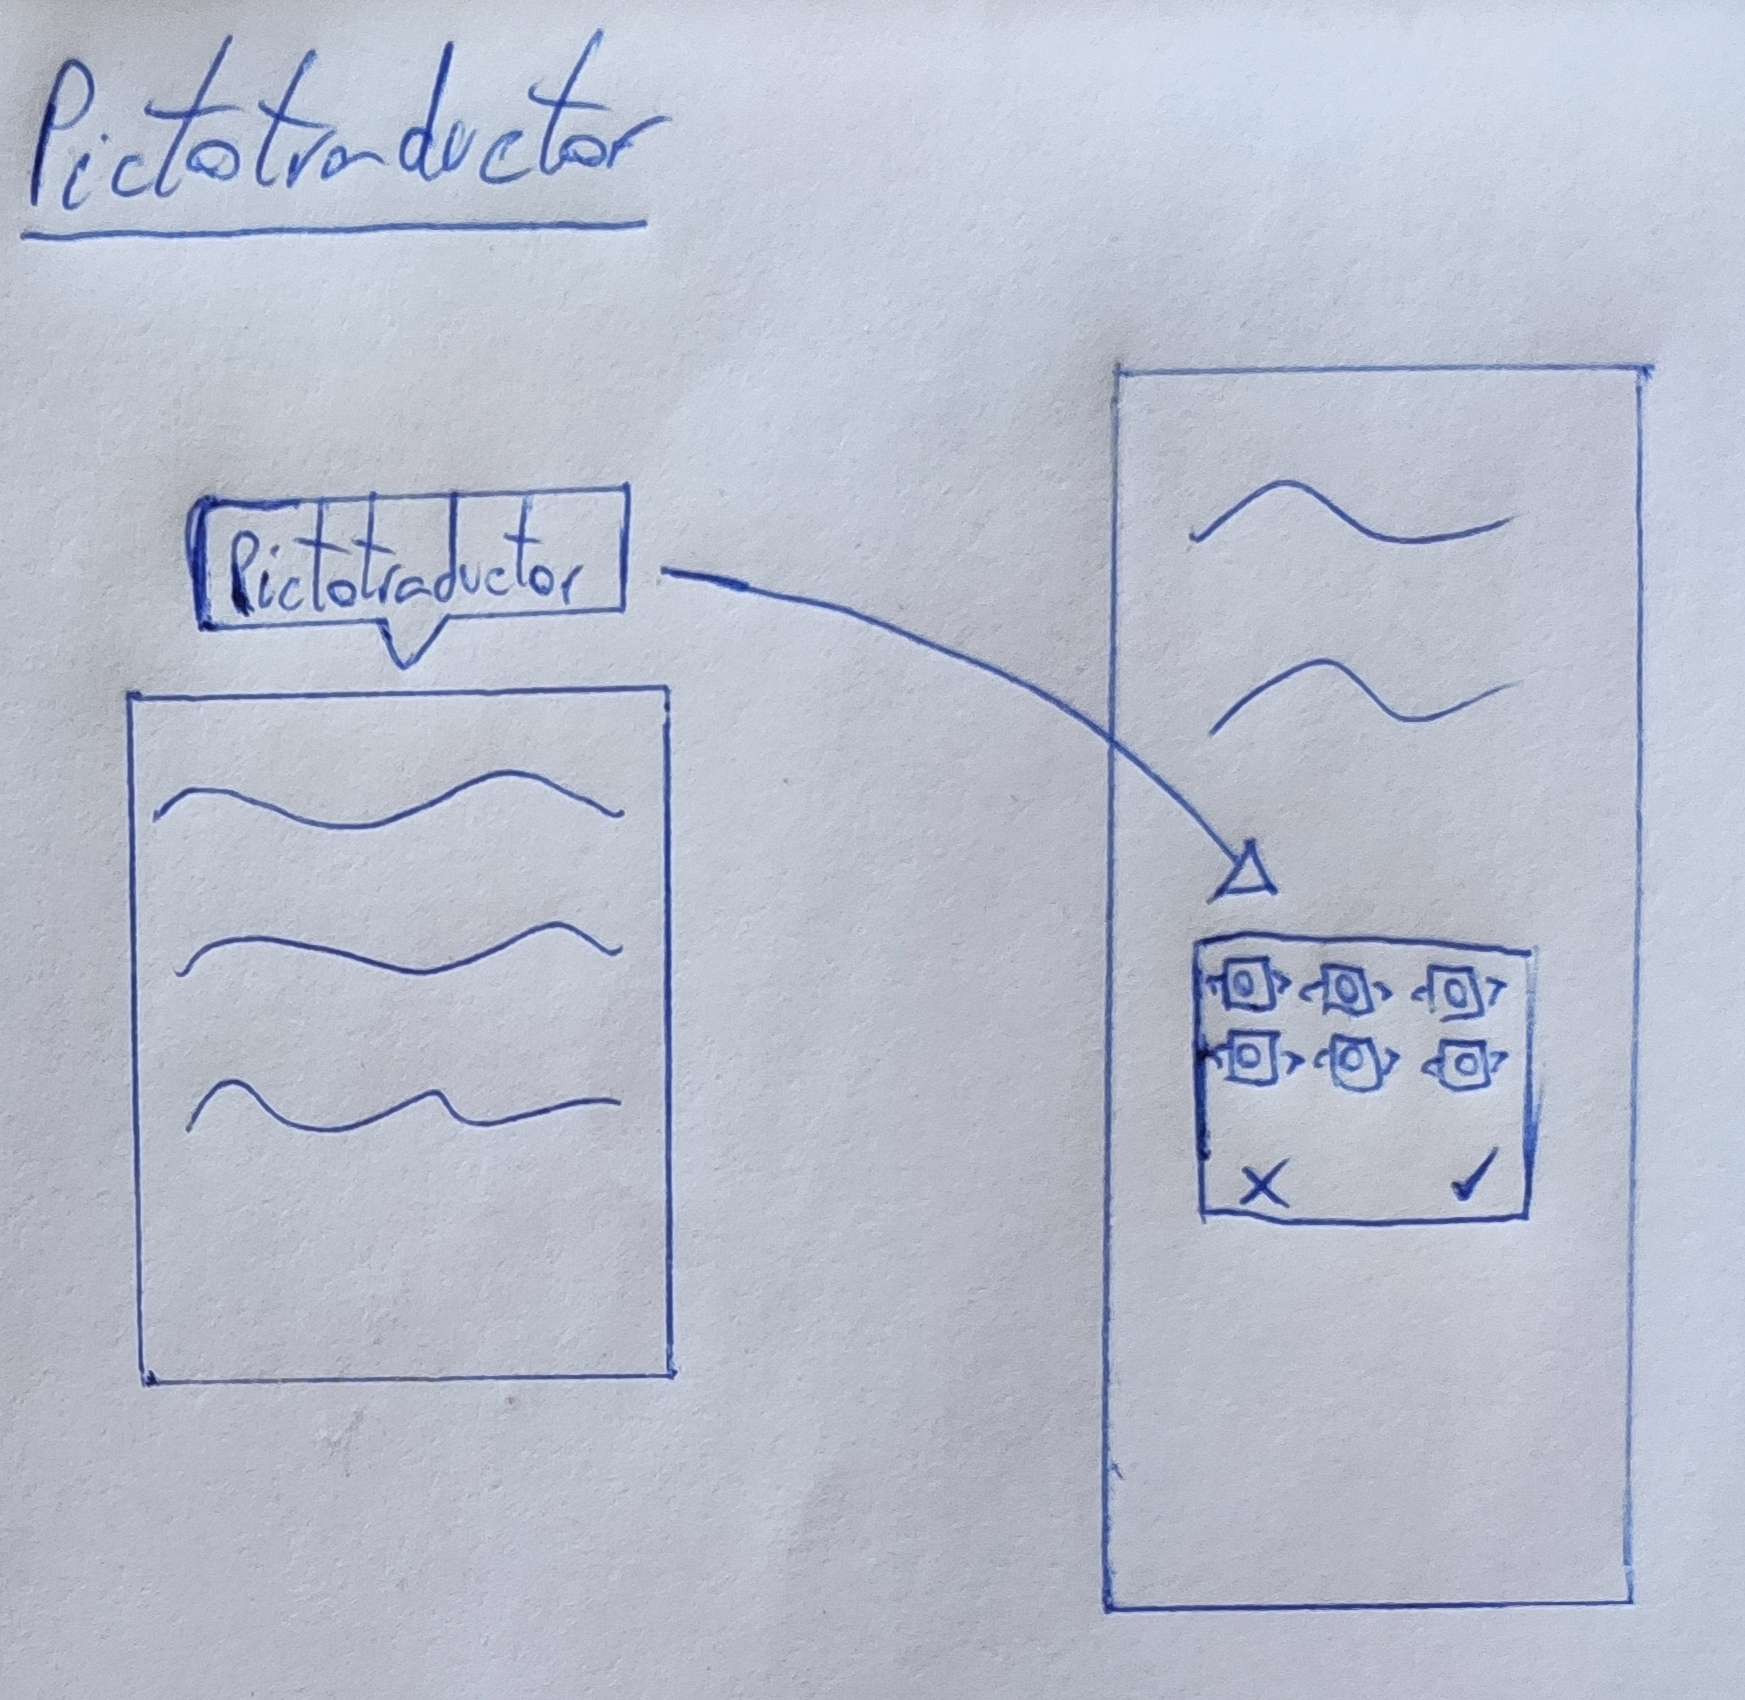
\includegraphics[width=10cm]{Diseño/Alvaro/Alvaro04.jpg}
  \caption{Diseño pictotraductor de Álvaro.}
  \label{fig:disenyoAlvaro04}
\end{figure}

\begin{figure}[ht!]
  \centering
  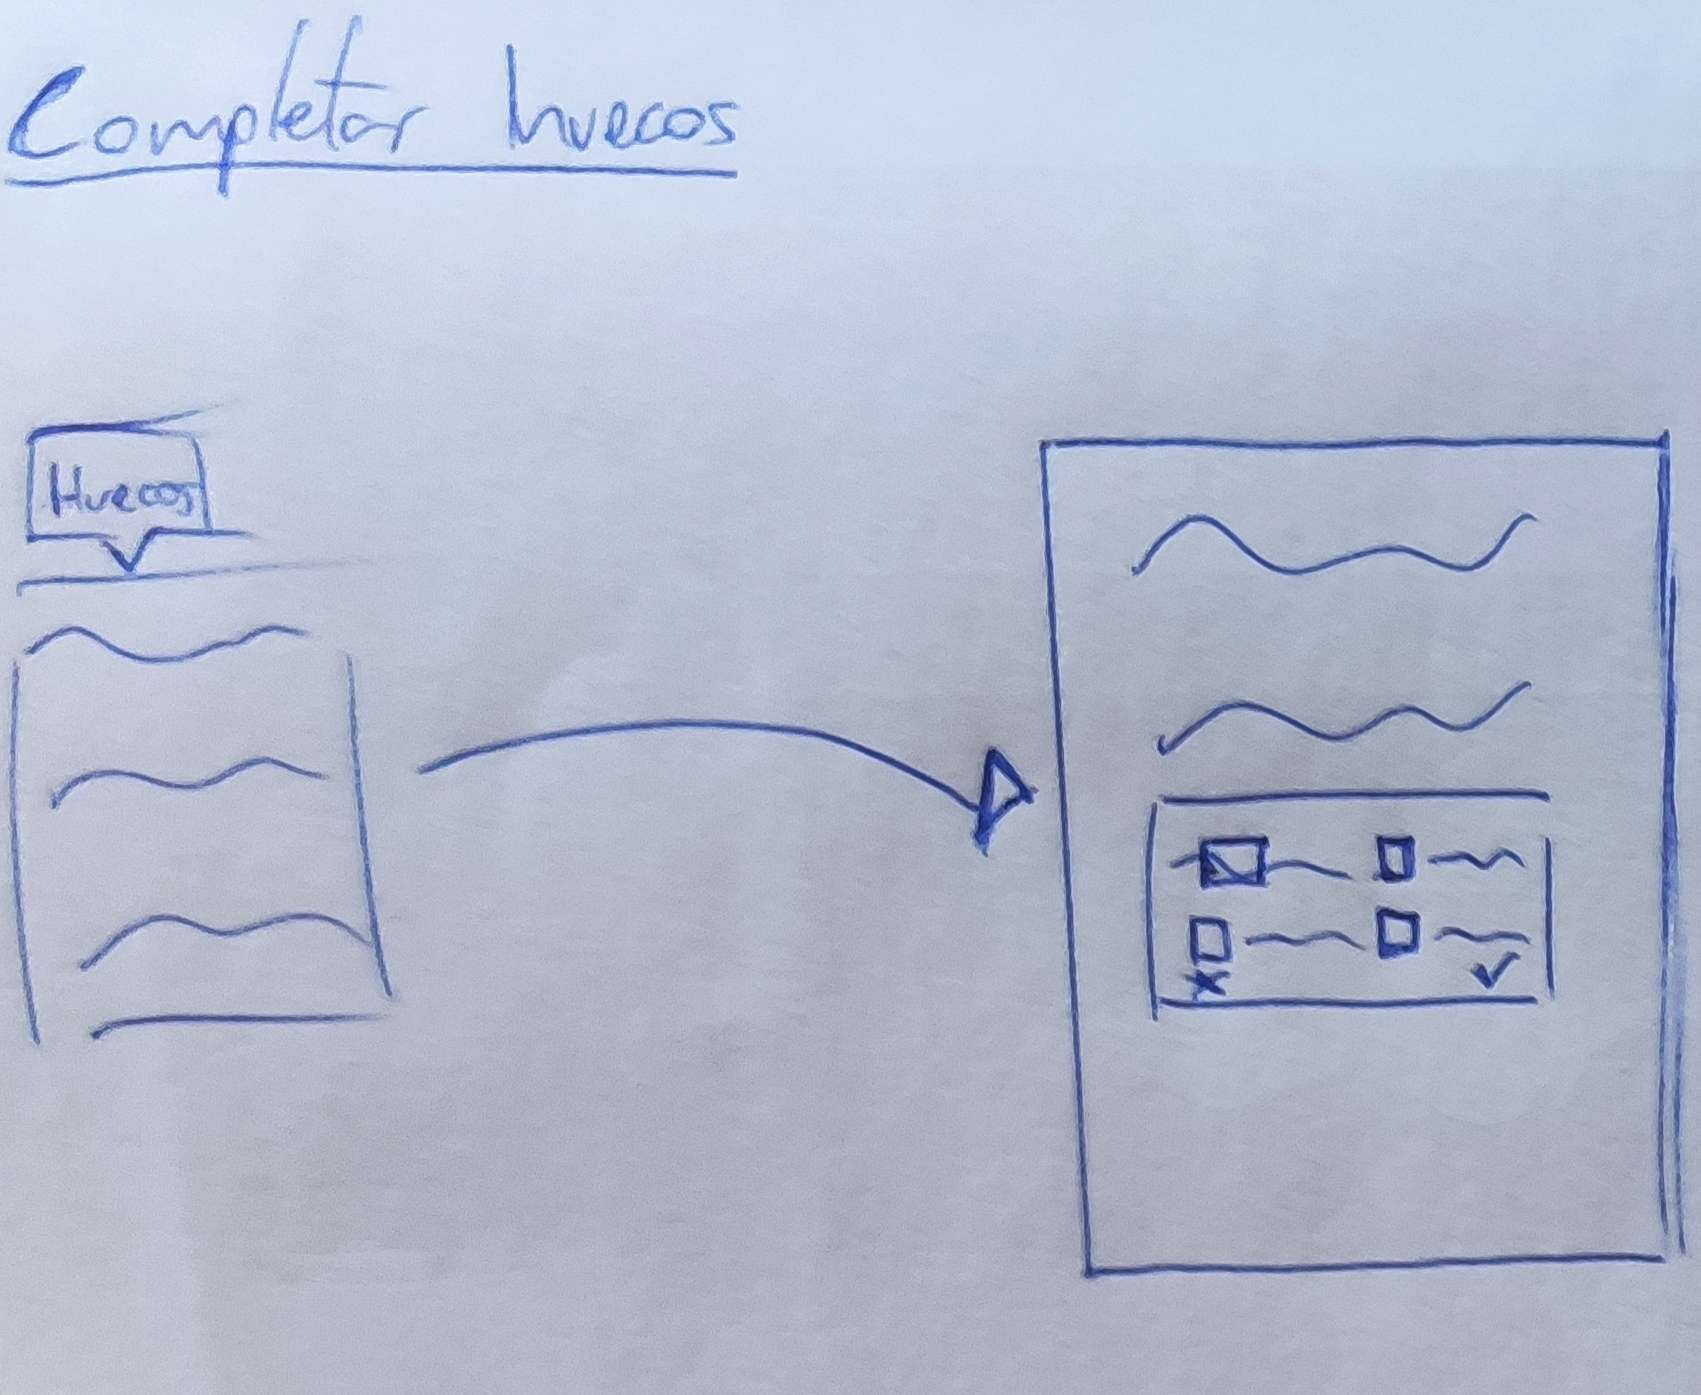
\includegraphics[width=10cm]{Diseño/Alvaro/Alvaro05.jpg}
  \caption{Diseño definir huecos de Álvaro.}
  \label{fig:disenyoAlvaro05}
\end{figure}

\begin{figure}[ht!]
  \centering
  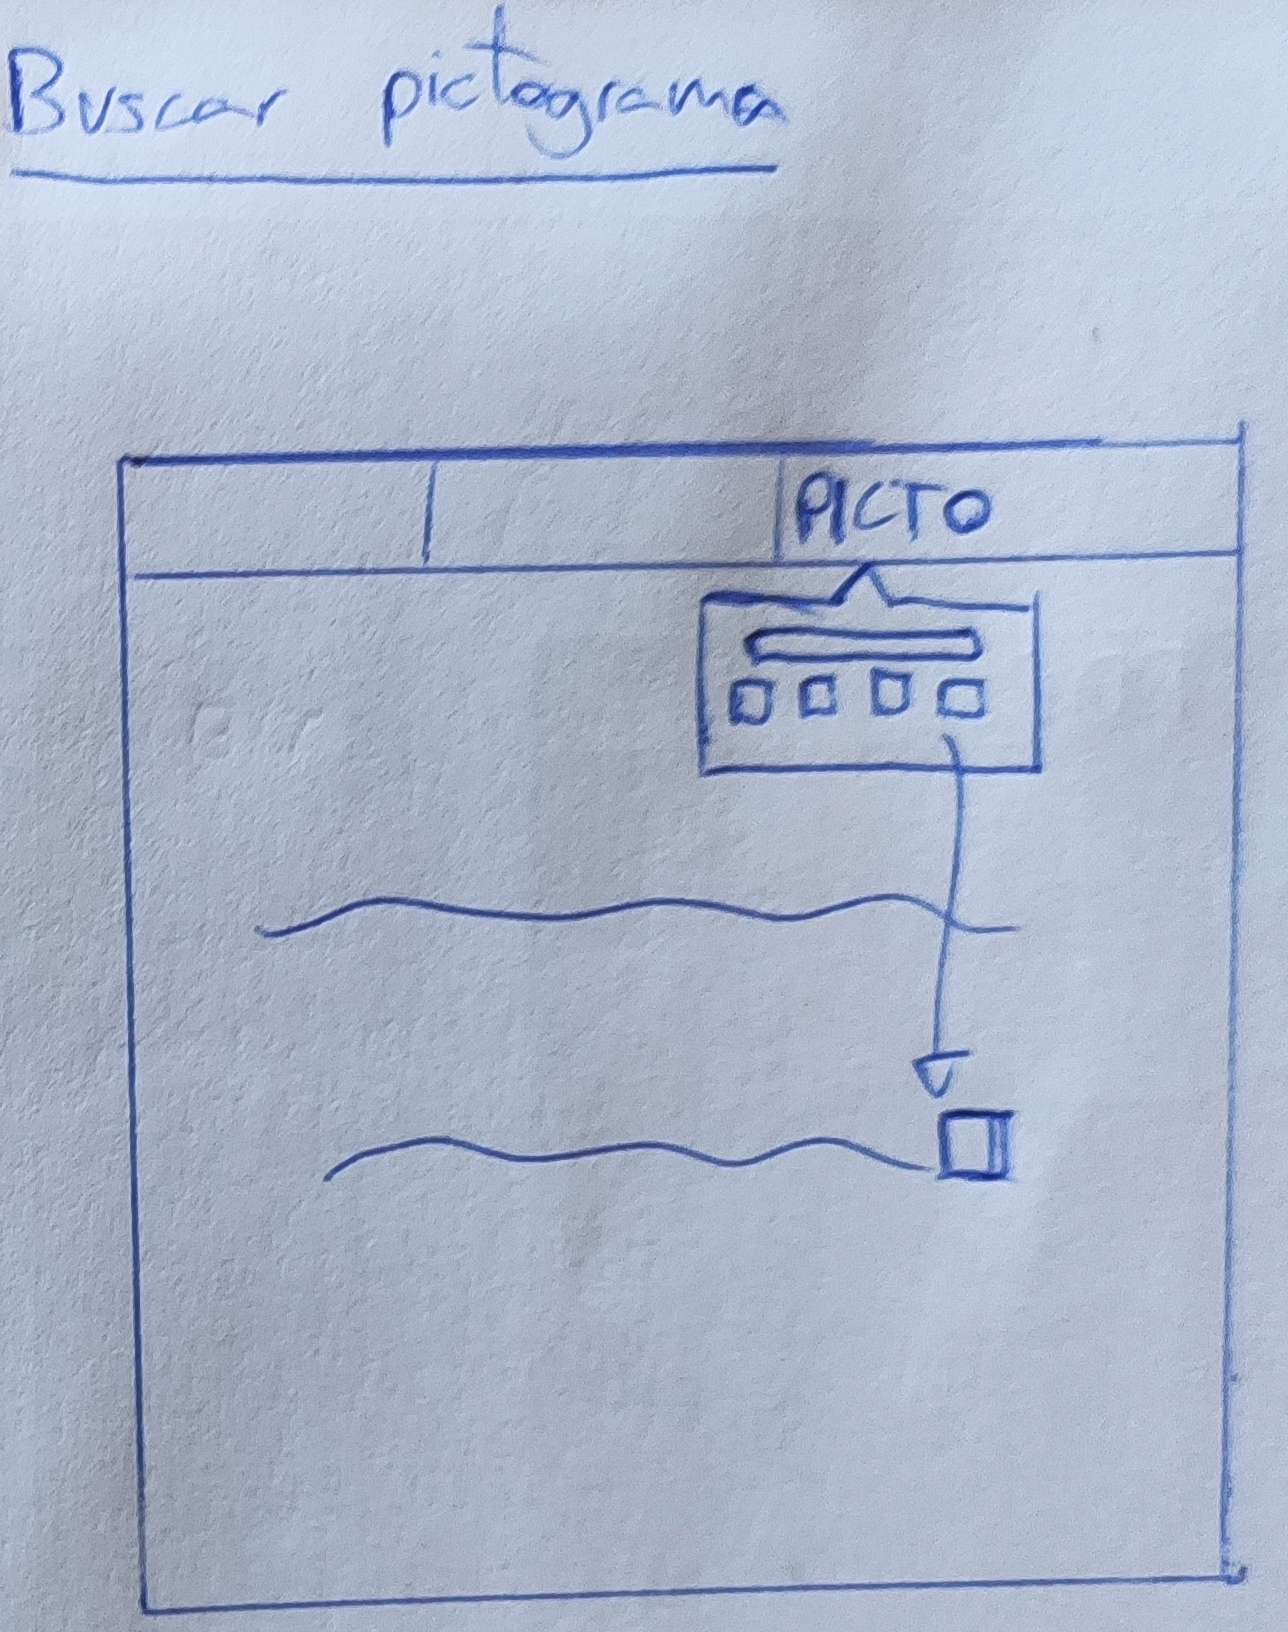
\includegraphics[width=10cm]{Diseño/Alvaro/Alvaro06.jpg}
  \caption{Diseño buscar pictogramas de Álvaro.}
  \label{fig:disenyoAlvaro06}
\end{figure}

\begin{figure}[ht!]
  \centering
  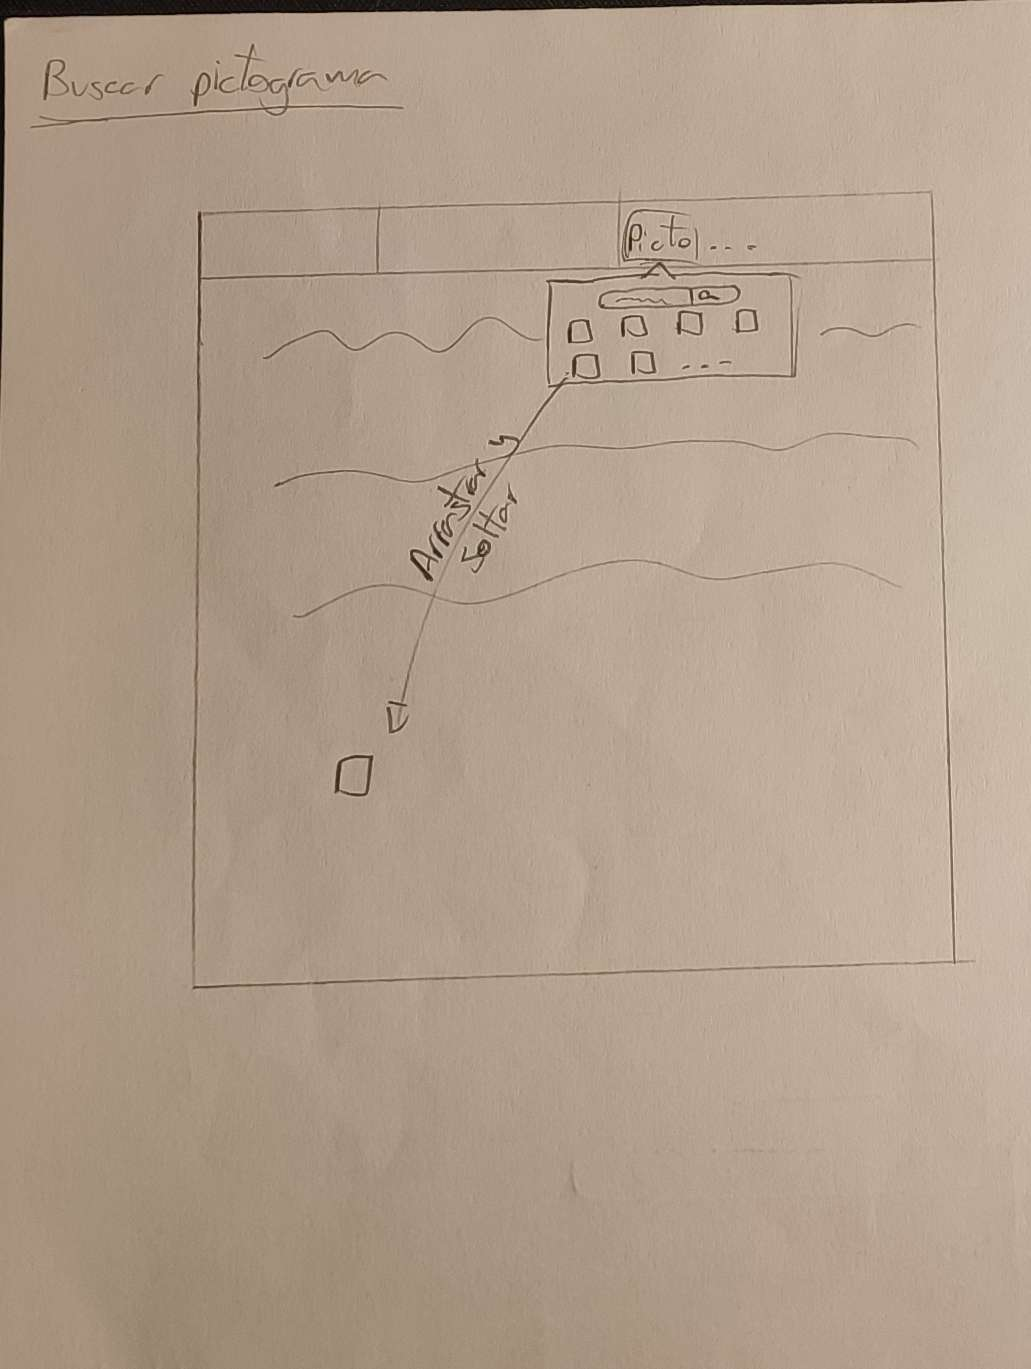
\includegraphics[width=10cm]{Diseño/Alvaro/Alvaro07.jpg}
  \caption{Diseño ejercicio de definiciones de Álvaro.}
  \label{fig:disenyoAlvaro07}
\end{figure}

\begin{figure}[ht!]
  \centering
  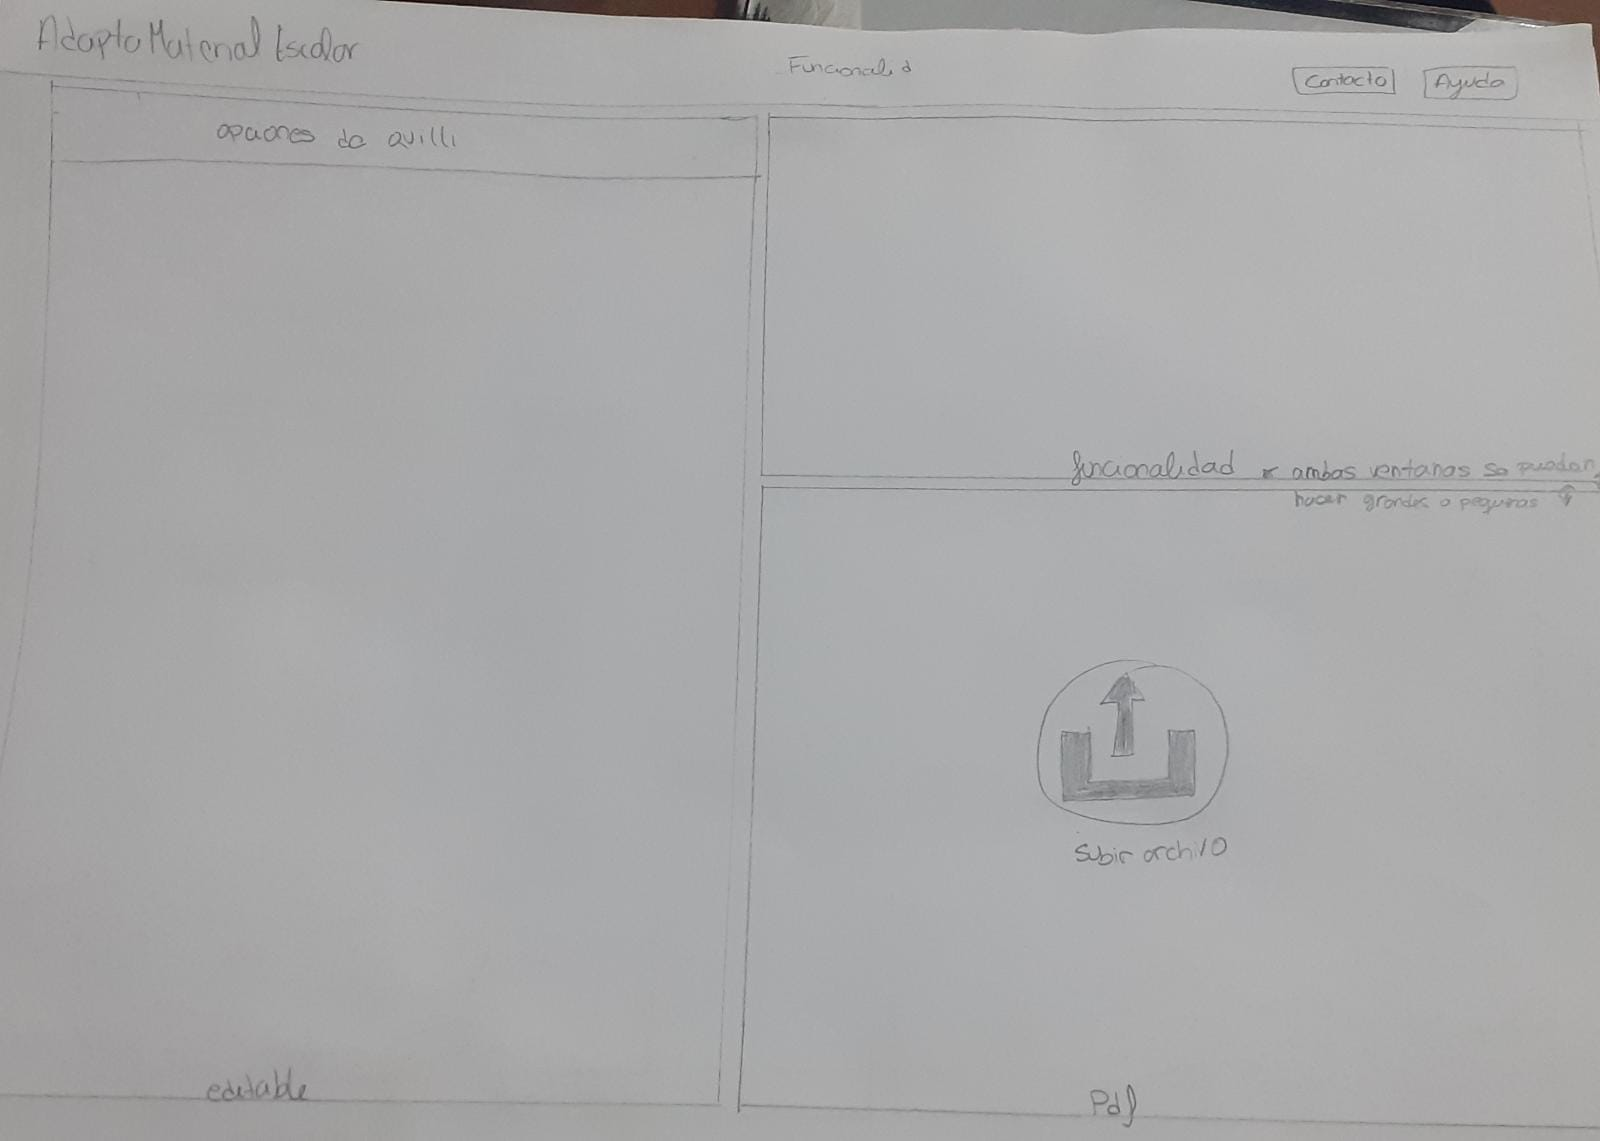
\includegraphics[width=15cm]{Diseño/Dunia/principal.jpeg}
  \caption{Diseño pantalla de inicio de Dunia.}
  \label{dunia1}
\end{figure}

\begin{figure}[ht!]
  \centering
  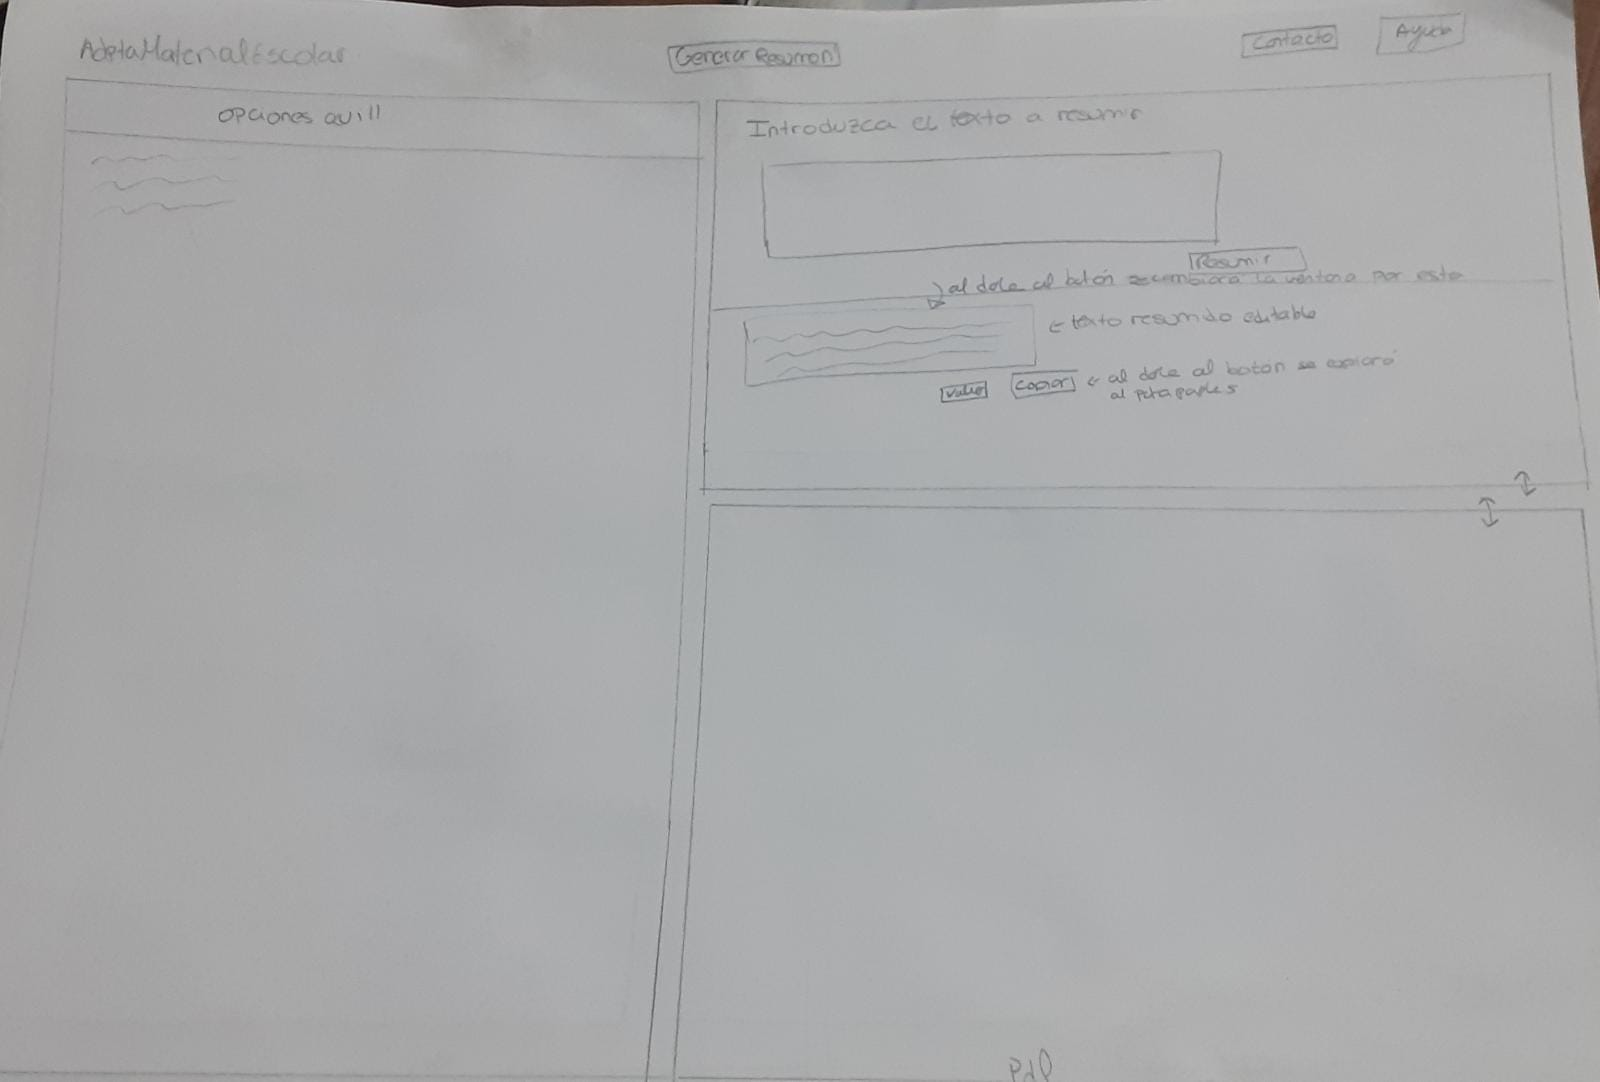
\includegraphics[width=15cm]{Diseño/Dunia/resumen.jpeg}
  \caption{Diseño pantalla de generar resumen de Dunia.}
  \label{dunia2}
\end{figure}

\begin{figure}[ht!]
  \centering
  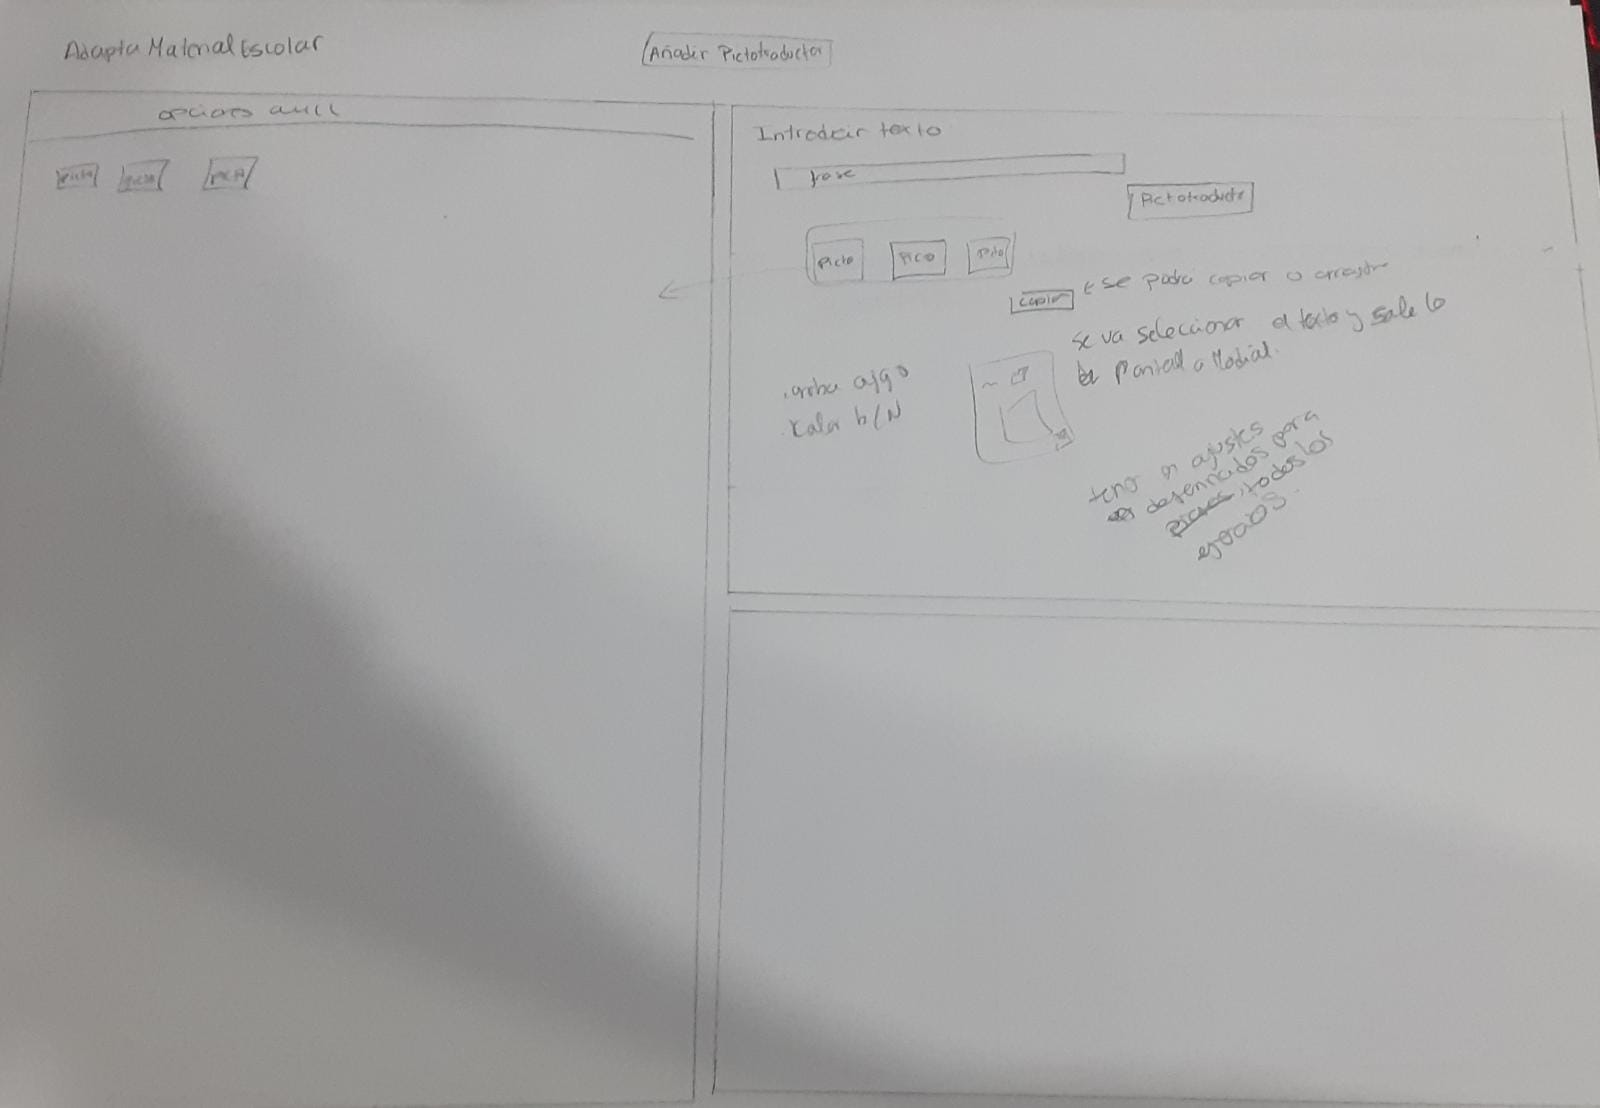
\includegraphics[width=15cm]{Diseño/Dunia/picto.jpeg}
  \caption{Diseño de pictotraductor de Dunia.}
  \label{dunia3}
\end{figure}

\begin{figure}[ht!]
  \centering
  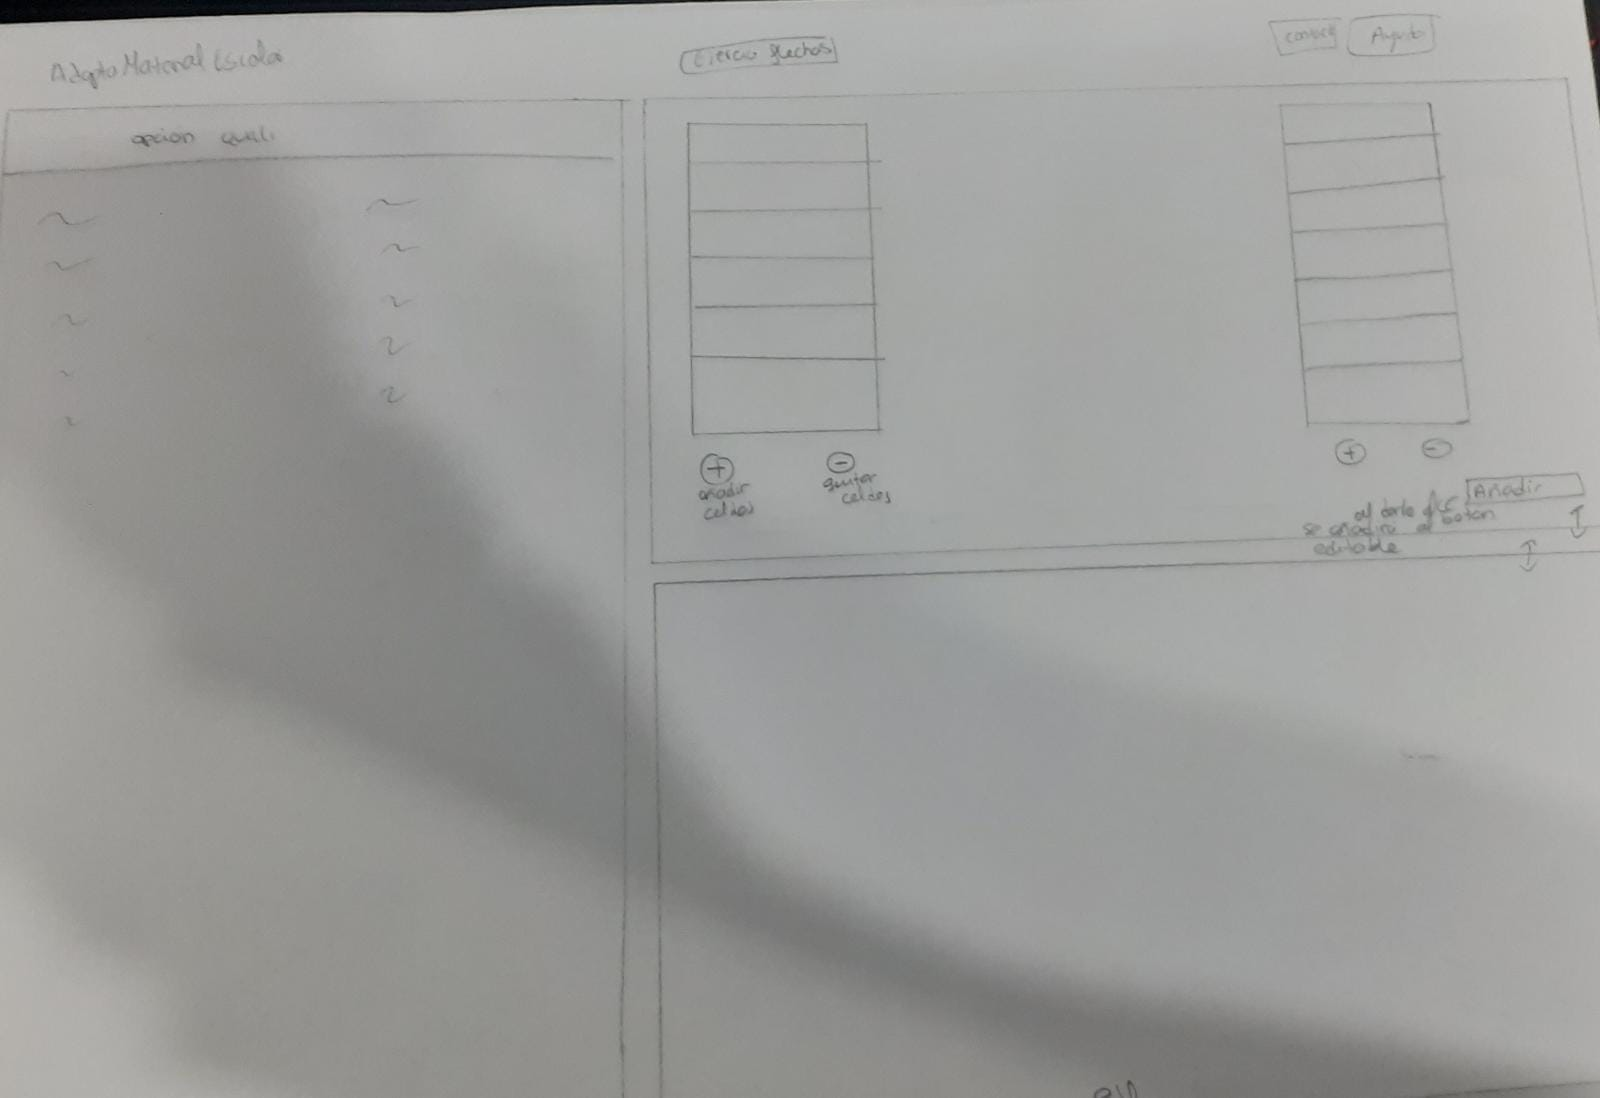
\includegraphics[width=15cm]{Diseño/Dunia/flechas.jpeg}
  \caption{Diseño de ejercicios de flechas de Dunia.}
  \label{dunia4}
\end{figure}

\begin{figure}[ht!]
  \centering
  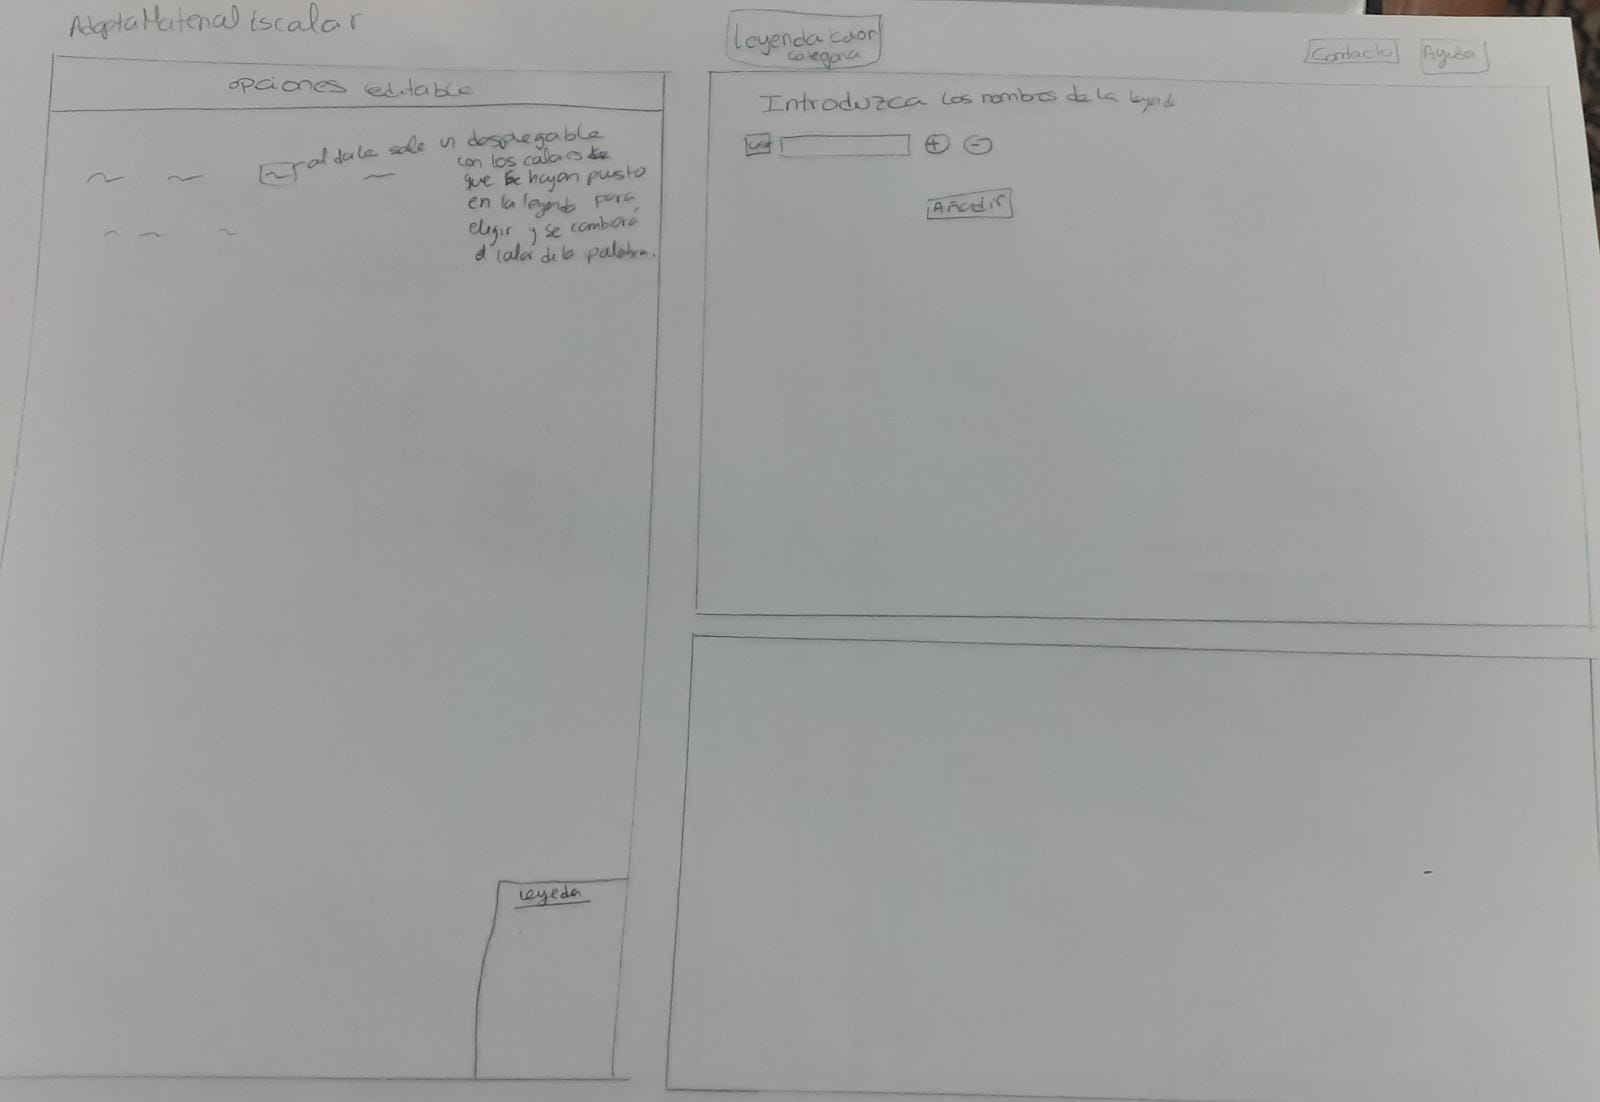
\includegraphics[width=15cm]{Diseño/Dunia/leyendaColor.jpeg}
  \caption{Diseño de leyenda de colores de Dunia.}
  \label{dunia5}
\end{figure}

\begin{figure}[ht!]
  \centering
  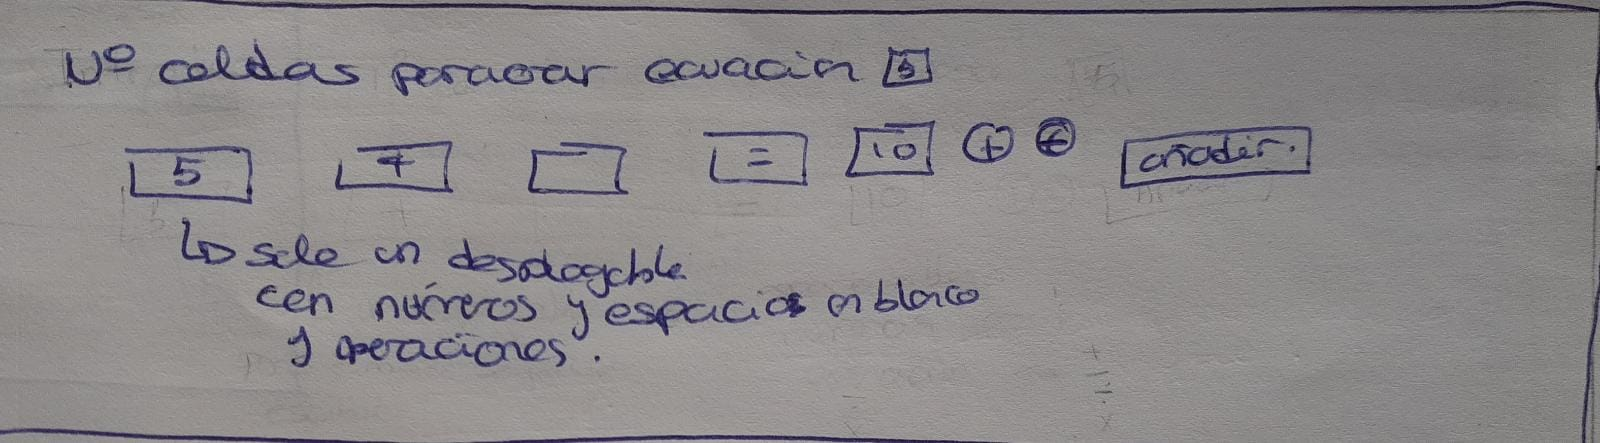
\includegraphics[width=15cm]{Diseño/Dunia/hueco.jpeg}
  \caption{Diseño de ejercicios matemáticas de huecos de Dunia.}
  \label{dunia6}
\end{figure}



\begin{figure}[ht!]
  \centering
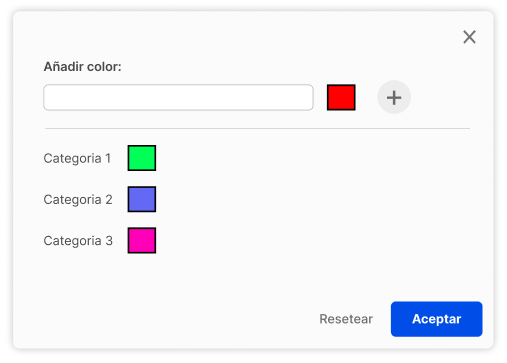
\includegraphics[width=15cm]{Diseño/Alberto/Capture01.PNG}
  \caption{Diseño de leyenda de colores de Alberto.}
\end{figure}

\begin{figure}[ht!]
  \centering
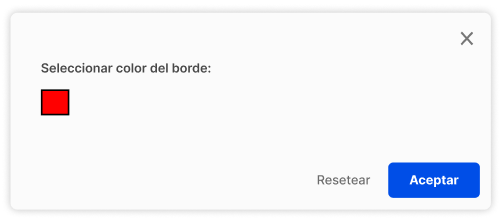
\includegraphics[width=15cm]{Diseño/Alberto/Capture02.PNG}
  \caption{Diseño de leyenda de colores por asignatura de Alberto.}
\end{figure}

\begin{figure}[ht!]
  \centering
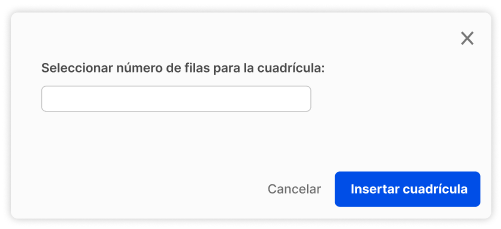
\includegraphics[width=15cm]{Diseño/Alberto/Capture03.PNG}
  \caption{Diseño de cuatrícula de Alberto.}
\end{figure}

\begin{figure}[ht!]
  \centering
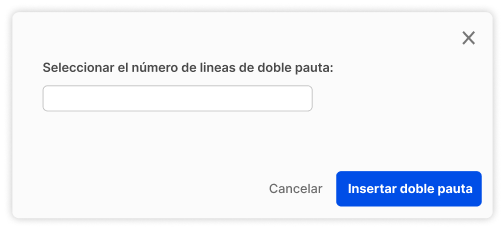
\includegraphics[width=15cm]{Diseño/Alberto/Capture04.PNG}
  \caption{Diseño de doble pauta de Alberto.}
\end{figure}

\begin{figure}[ht!]
  \centering
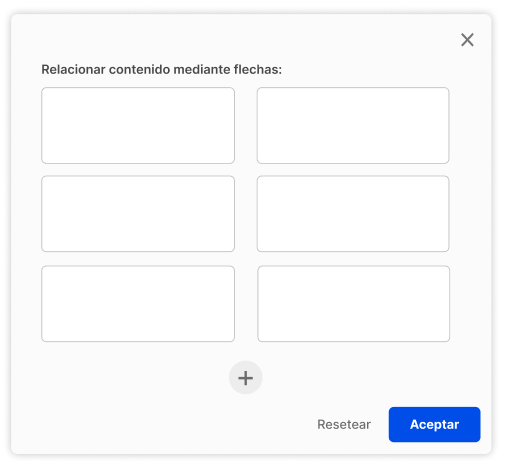
\includegraphics[width=15cm]{Diseño/Alberto/Capture05.PNG}
  \caption{Diseño de ejercicio de flechas de Alberto.}
\end{figure}

\begin{figure}[ht!]
  \centering
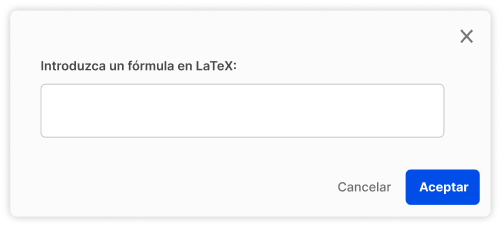
\includegraphics[width=15cm]{Diseño/Alberto/Capture06.PNG}
  \caption{Diseño de ejercicios de matemáticas con huecos de Alberto.}
\end{figure}

\begin{figure}[ht!]
  \centering
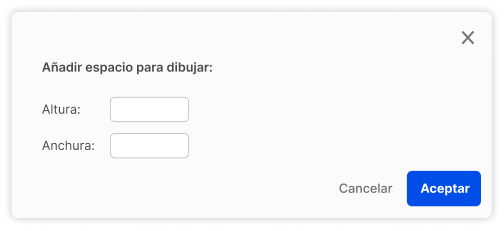
\includegraphics[width=15cm]{Diseño/Alberto/Capture07.PNG}
  \caption{Diseño de ejercicios de espacios para dibujar de Alberto.}
\end{figure}

\begin{figure}[ht!]
  \centering
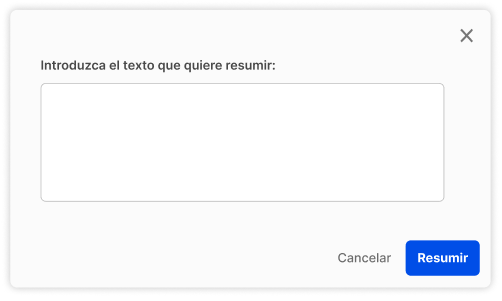
\includegraphics[width=15cm]{Diseño/Alberto/Capture08.PNG}
  \caption{Diseño de añadir resumen de Alberto.}
\end{figure}

\begin{figure}[ht!]
  \centering
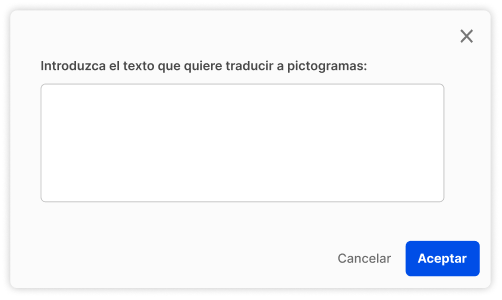
\includegraphics[width=15cm]{Diseño/Alberto/Capture10.PNG}
  \caption{Diseño de pictotraductor de Alberto.}
\end{figure}

\begin{figure}[ht!]
  \centering
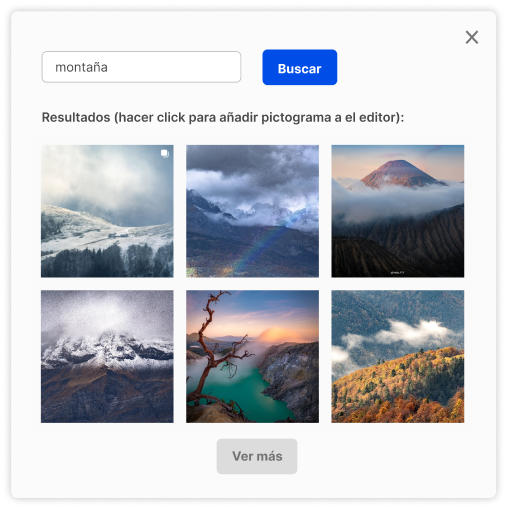
\includegraphics[width=15cm]{Diseño/Alberto/Capture12.PNG}
  \caption{Diseño de buscar pictogramas de Alberto.}
\end{figure}

\begin{figure}[ht!]
  \centering
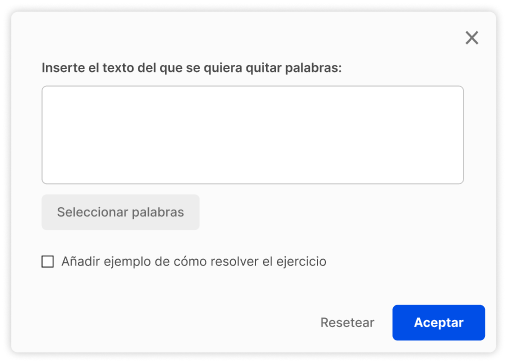
\includegraphics[width=15cm]{Diseño/Alberto/Capture13.PNG}
  \caption{Diseño de ejercicios con huecos de Alberto.}
\end{figure}

\begin{figure}[ht!]
  \centering
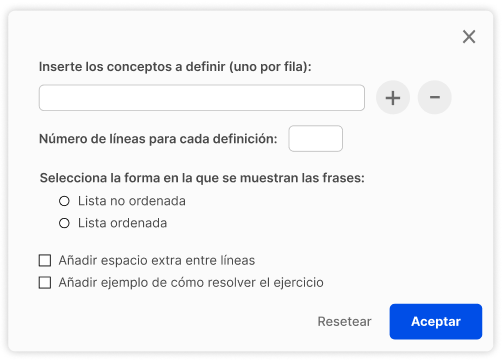
\includegraphics[width=15cm]{Diseño/Alberto/Capture14.PNG}
  \caption{Diseño de ejercicios de definiciones de Alberto.}
\end{figure}

\begin{figure}[ht!]
  \centering
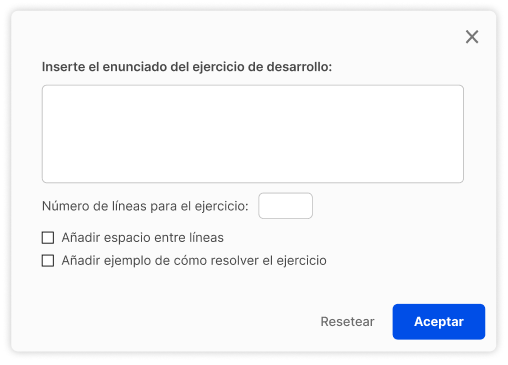
\includegraphics[width=15cm]{Diseño/Alberto/Capture15.PNG}
  \caption{Diseño de ejercicios de desarrollo de Alberto.}
\end{figure}

\begin{figure}[ht!]
  \centering
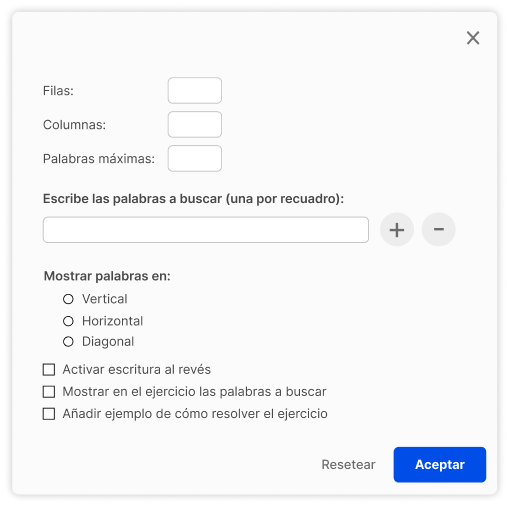
\includegraphics[width=15cm]{Diseño/Alberto/Capture16.PNG}
  \caption{Diseño de ejercicios de sopa de letras de Alberto.}
\end{figure}

\begin{figure}[ht!]
  \centering
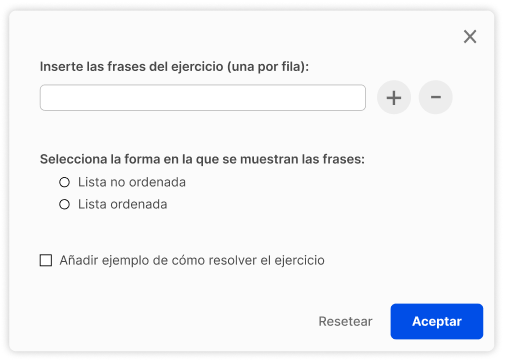
\includegraphics[width=15cm]{Diseño/Alberto/Capture17.PNG}
  \caption{Diseño de ejercicios de verdadero y falso de Alberto.}
\end{figure}





\begin{figure}[ht!]
  \centering
  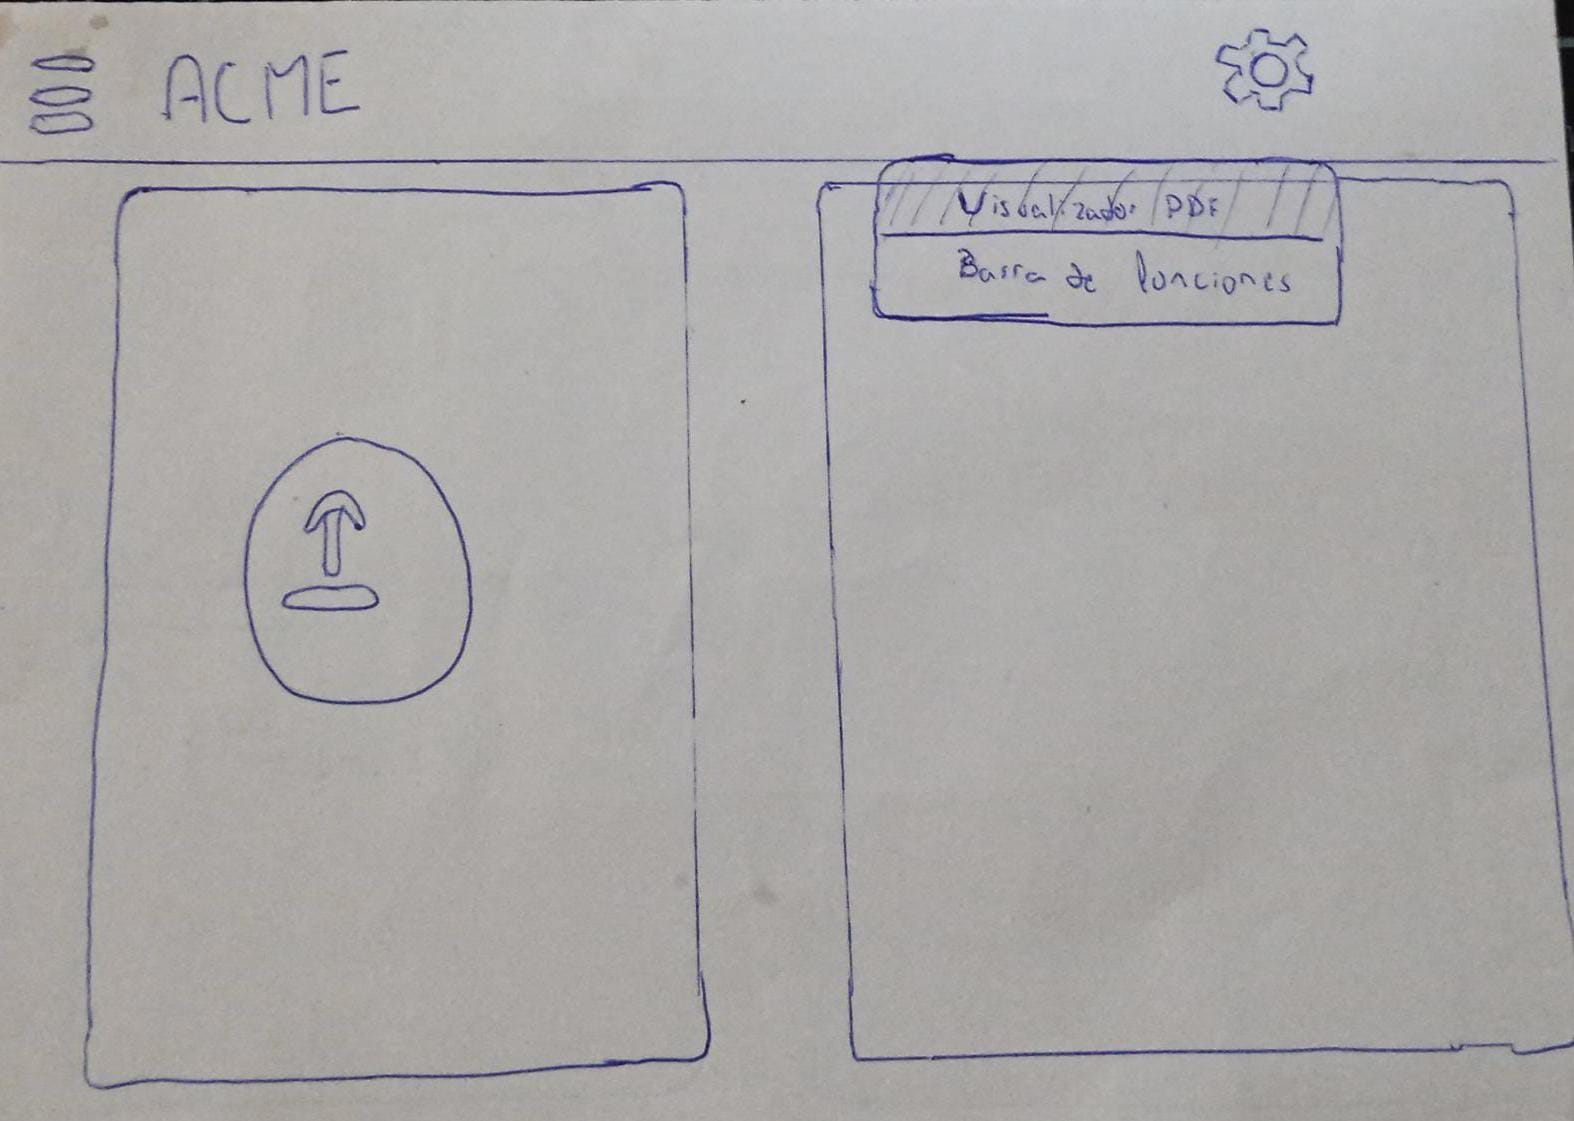
\includegraphics[width=15cm]{Diseño/Johan/Johan10.jpeg}
  \caption{Diseño pantalla de inicio de Johan.}
  \label{Johan10}
\end{figure}

\begin{figure}[ht!]
  \centering
  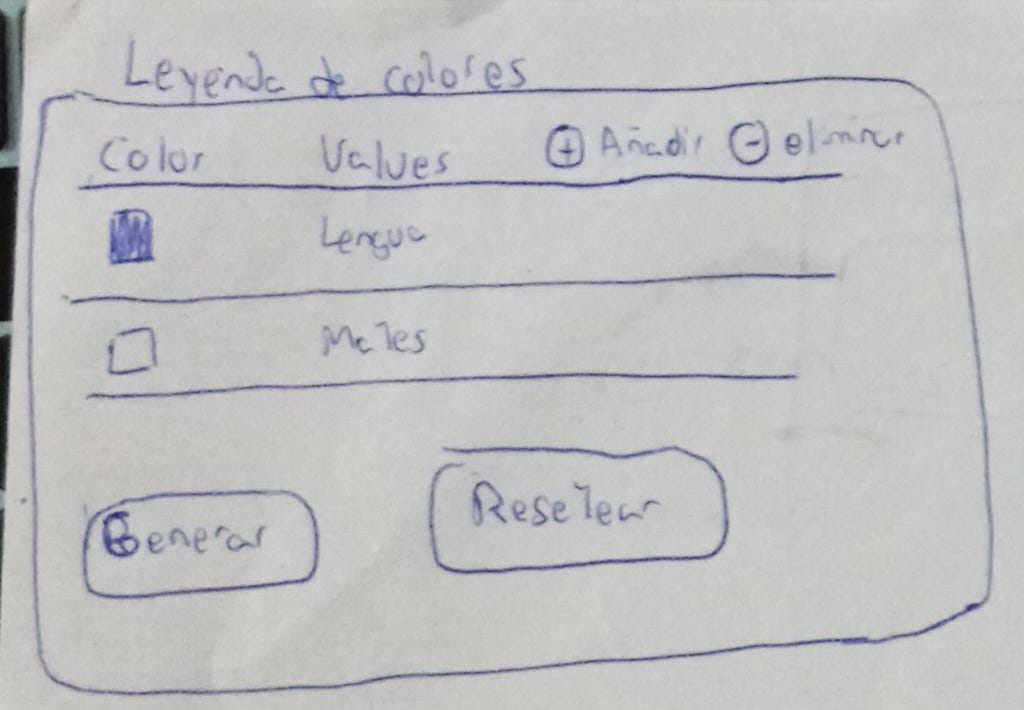
\includegraphics[width=15cm]{Diseño/Johan/Johan9.jpeg}
  \caption{Diseño pantalla de inicio completa de Johan.}
  \label{Johan9}
\end{figure}

\begin{figure}[ht!]
  \centering
  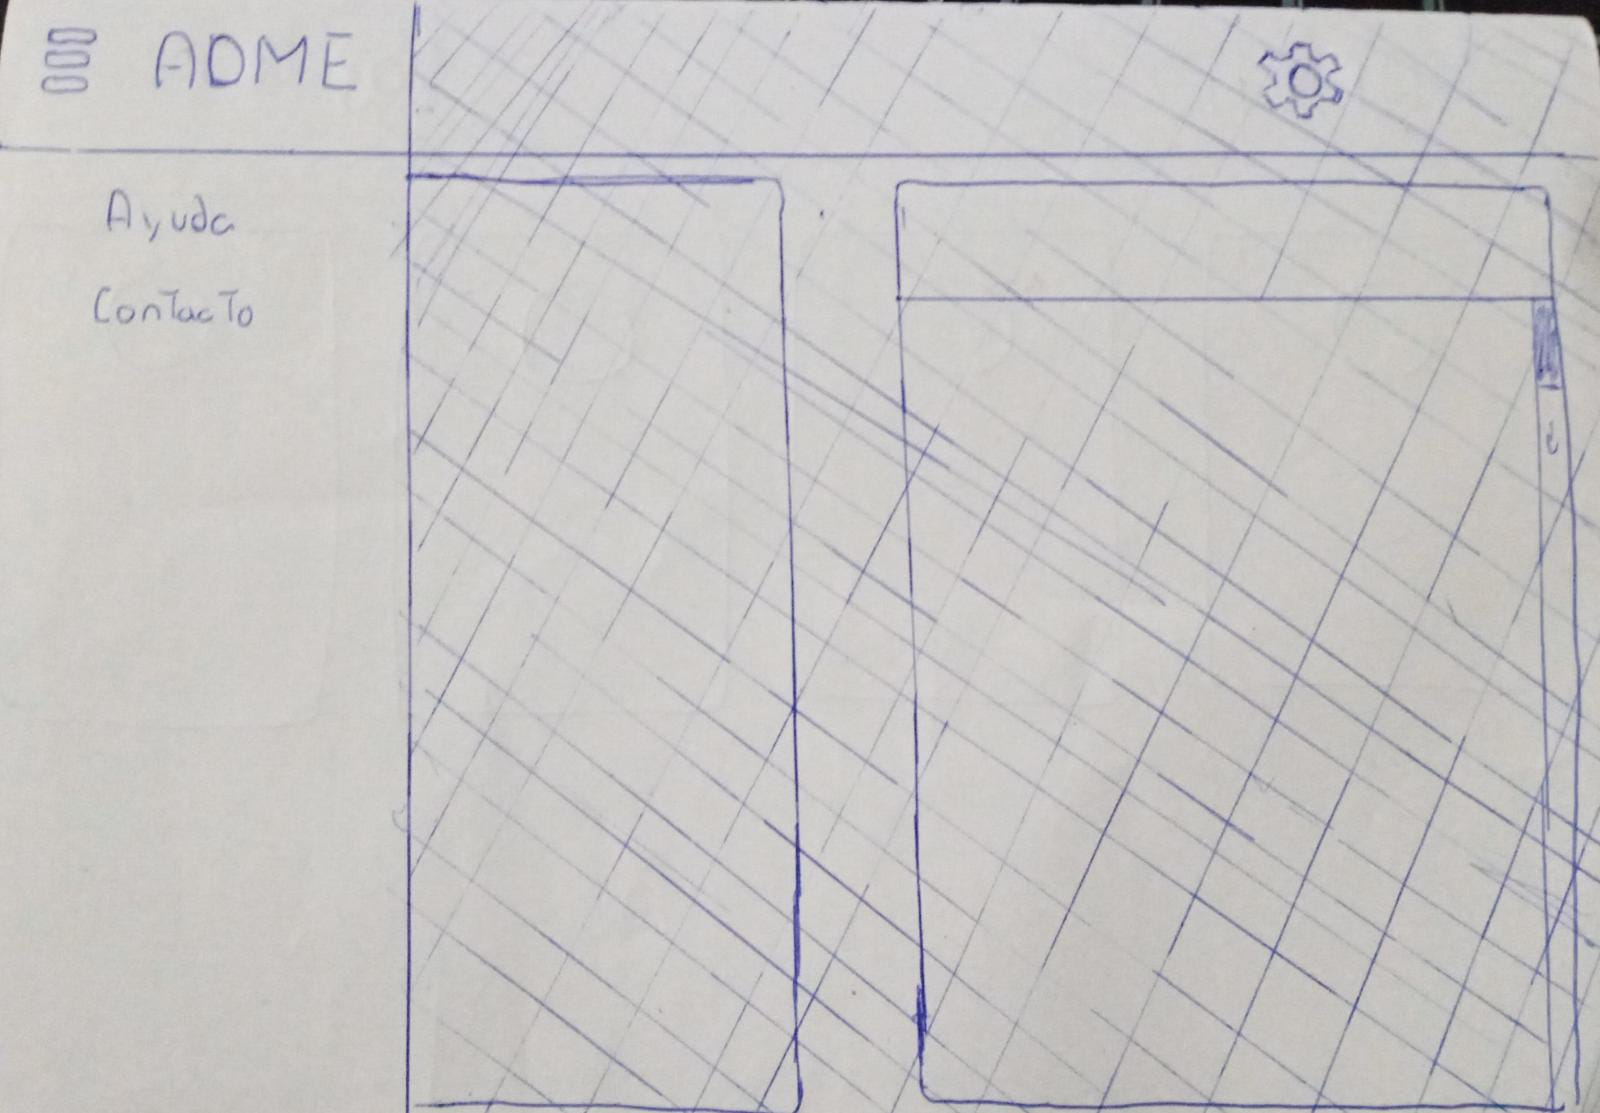
\includegraphics[width=15cm]{Diseño/Johan/Johan7.jpeg}
  \caption{Diseño de barra de navegación de Johan.}
  \label{Johan7}
\end{figure}

\begin{figure}[ht!]
  \centering
  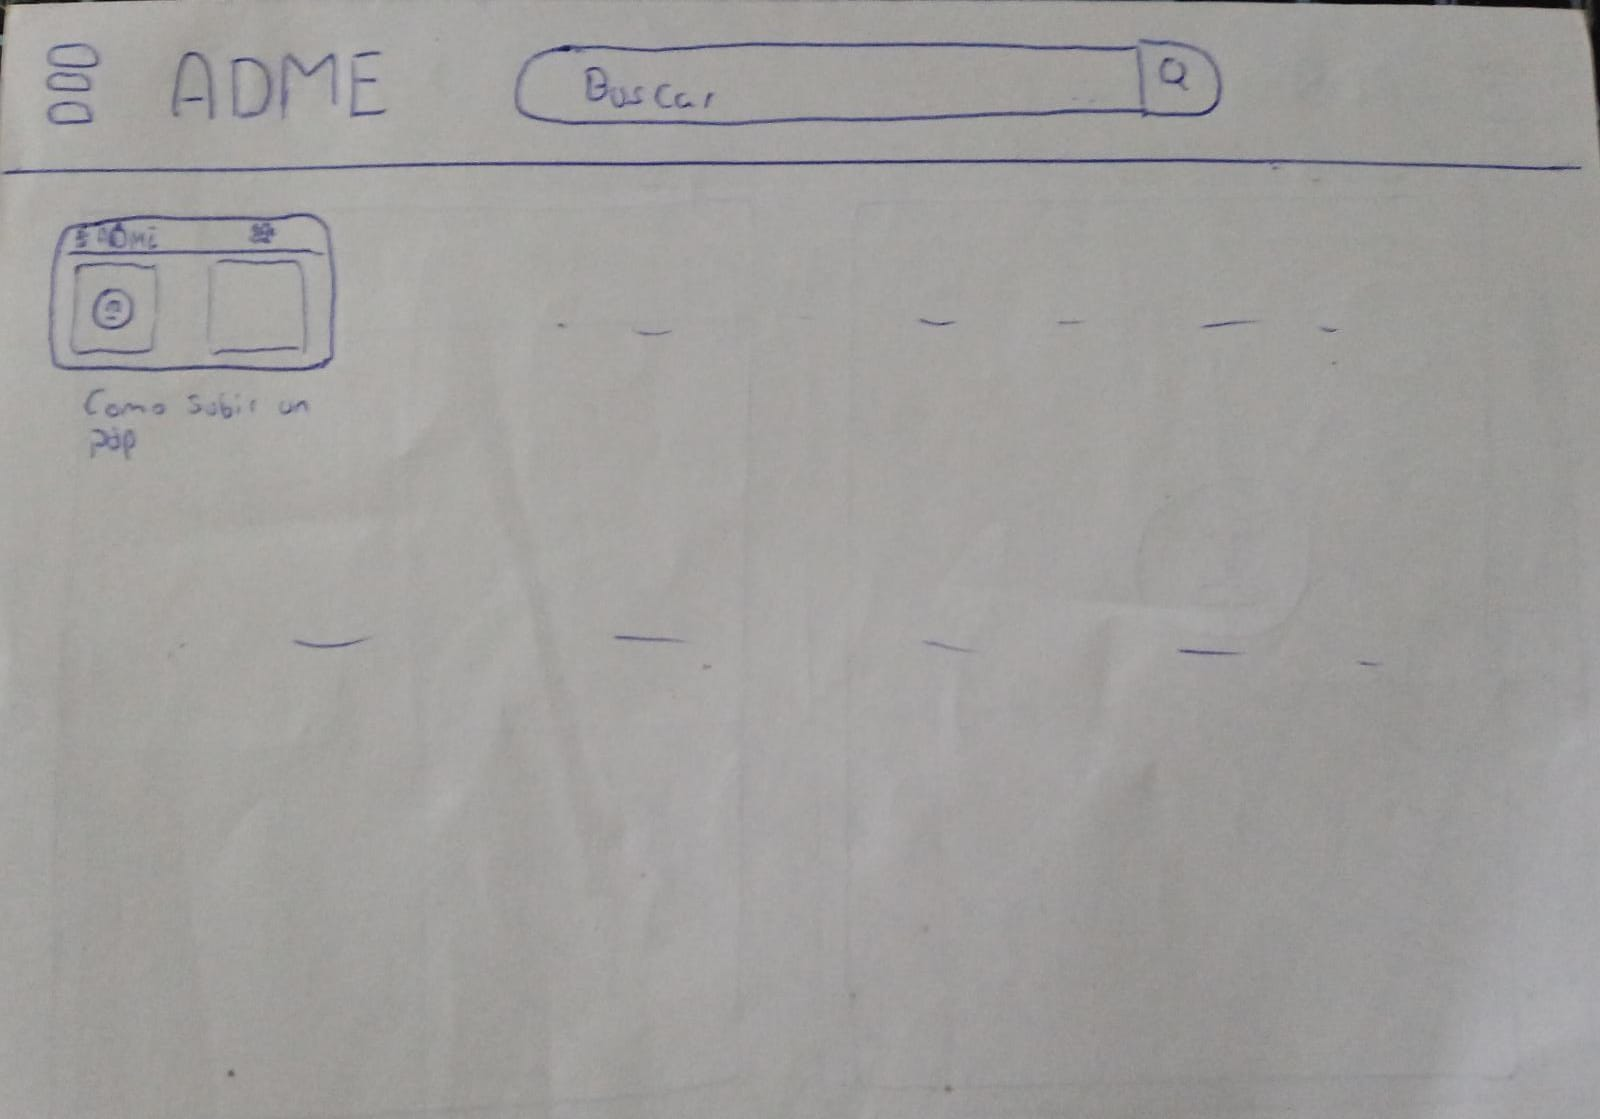
\includegraphics[width=15cm]{Diseño/Johan/Johan11.jpeg}
  \caption{Diseño de página de información de Johan.}
  \label{Johan11}
\end{figure}

\begin{figure}[ht!]
  \centering
  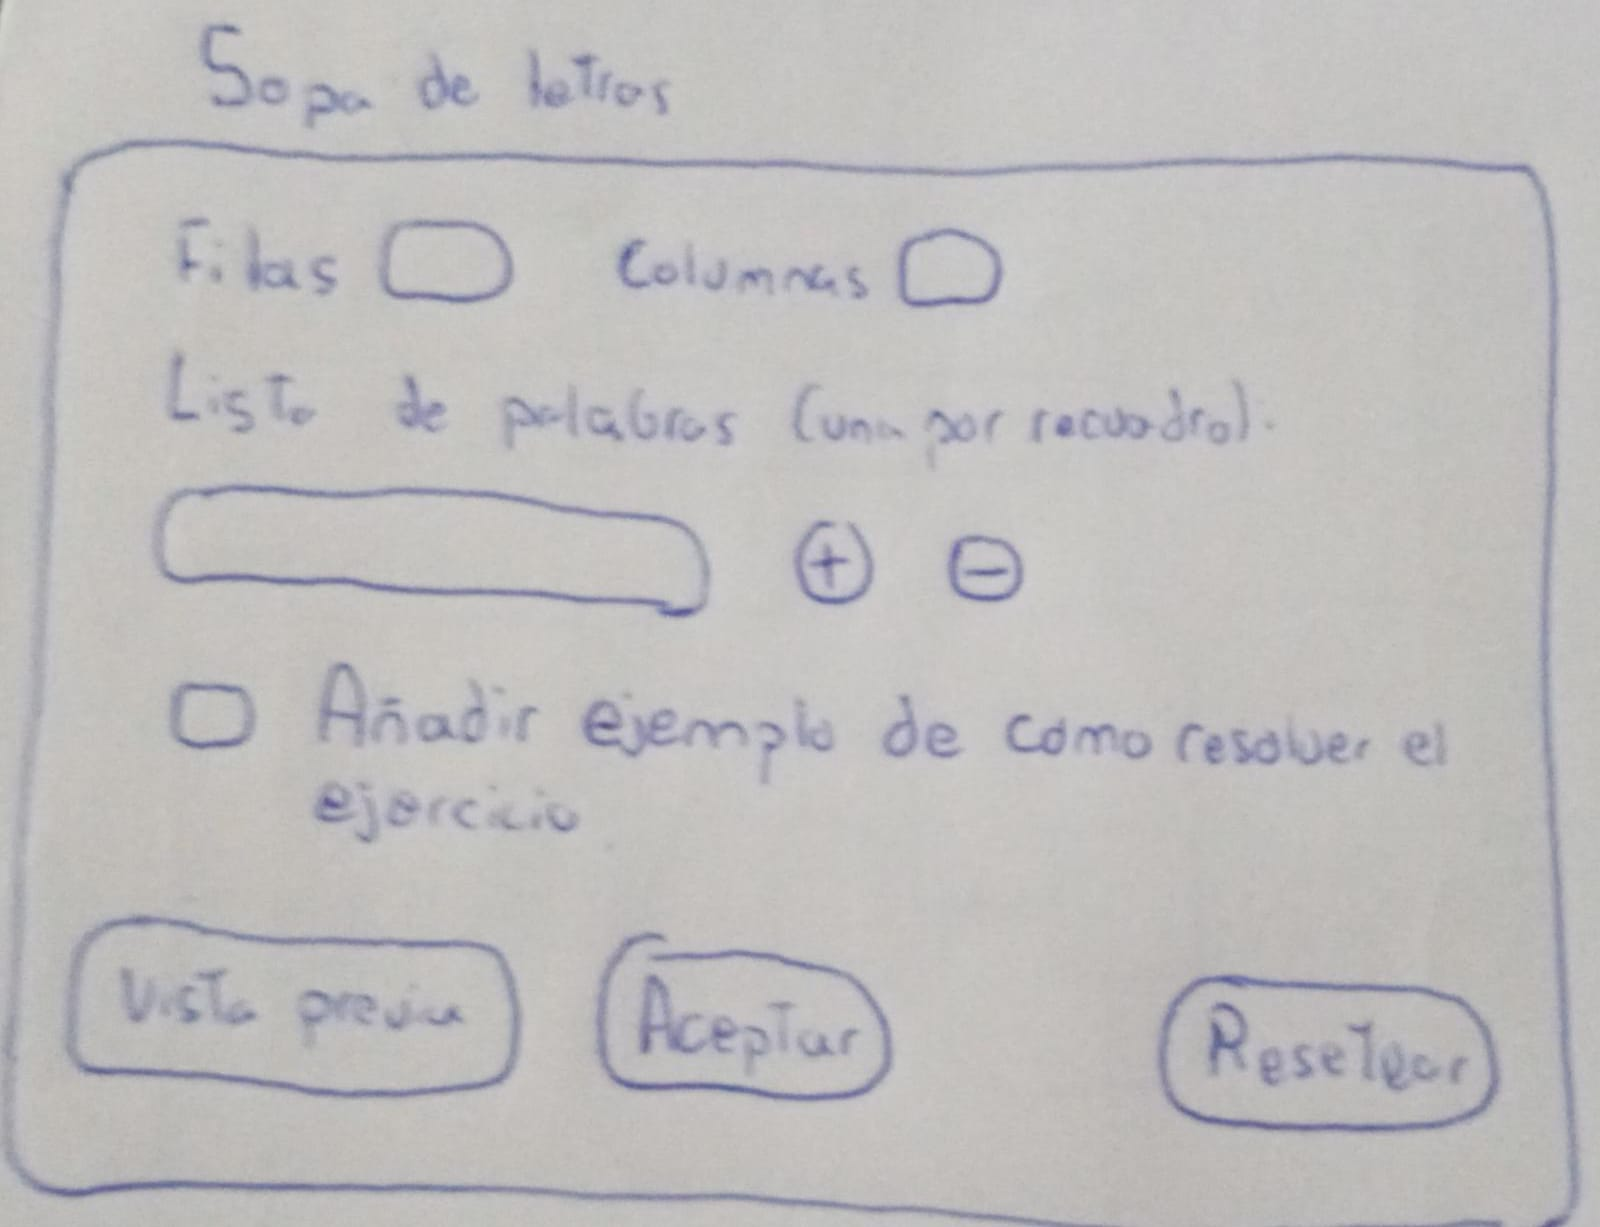
\includegraphics[width=15cm]{Diseño/Johan/Johan6.jpeg}
  \caption{Diseño de página de sobre nosotros de Johan.}
  \label{Johan6}
\end{figure}

\begin{figure}[ht!]
  \centering
  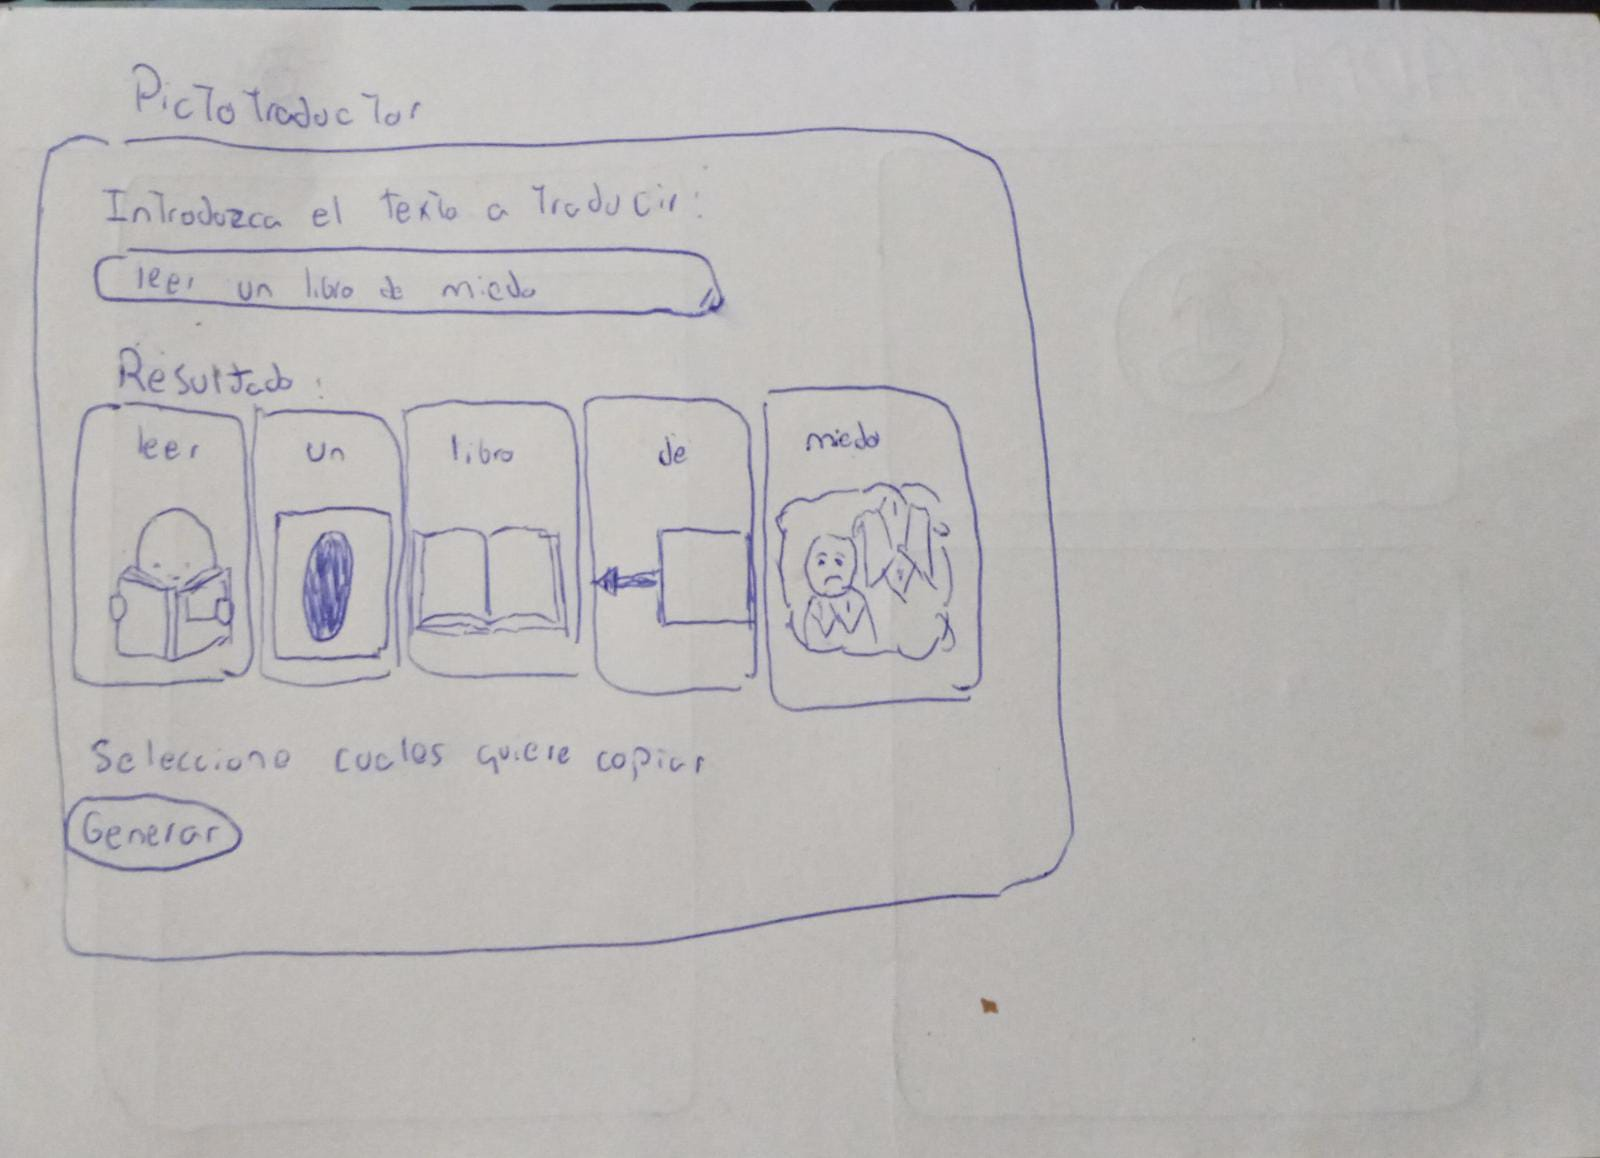
\includegraphics[width=15cm]{Diseño/Johan/Johan4.jpeg}
  \caption{Diseño de pictotraductor de Johan.}
  \label{Johan4}
\end{figure}

\begin{figure}[ht!]
  \centering
  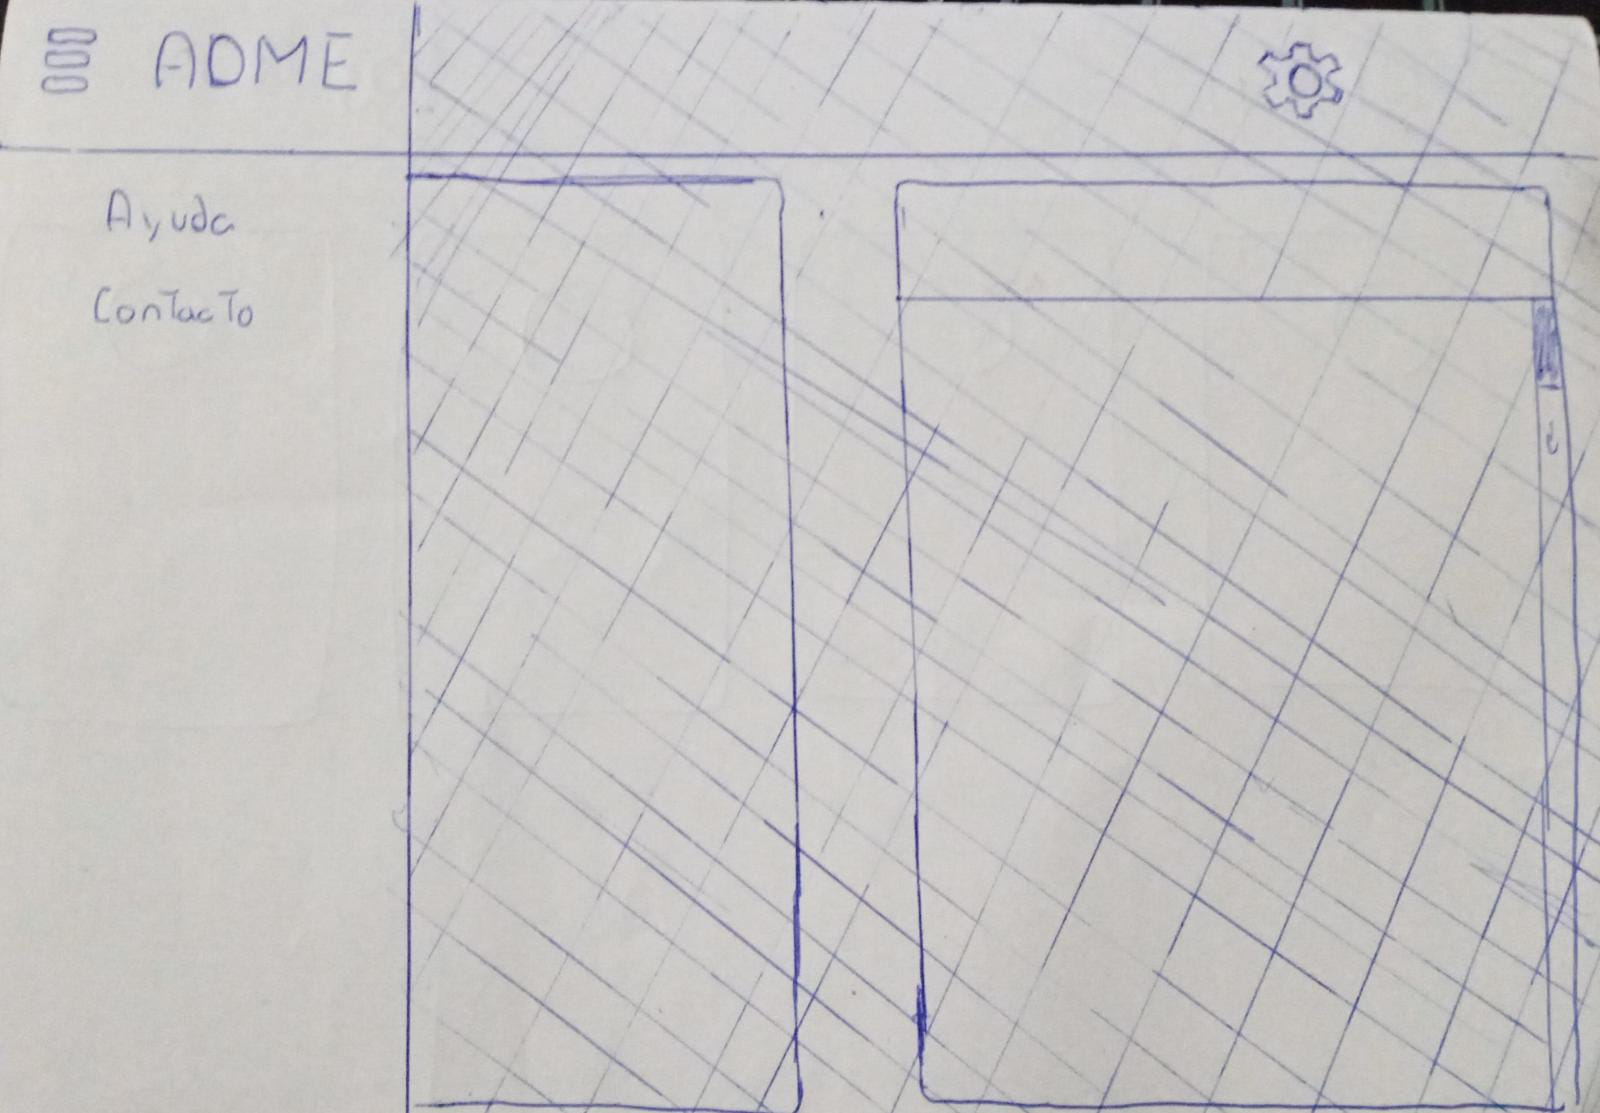
\includegraphics[width=15cm]{Diseño/Johan/Johan3.jpeg}
  \caption{Diseño de ejercicios de flechas de Johan.}
  \label{Johan3}
\end{figure}

\begin{figure}[ht!]
  \centering

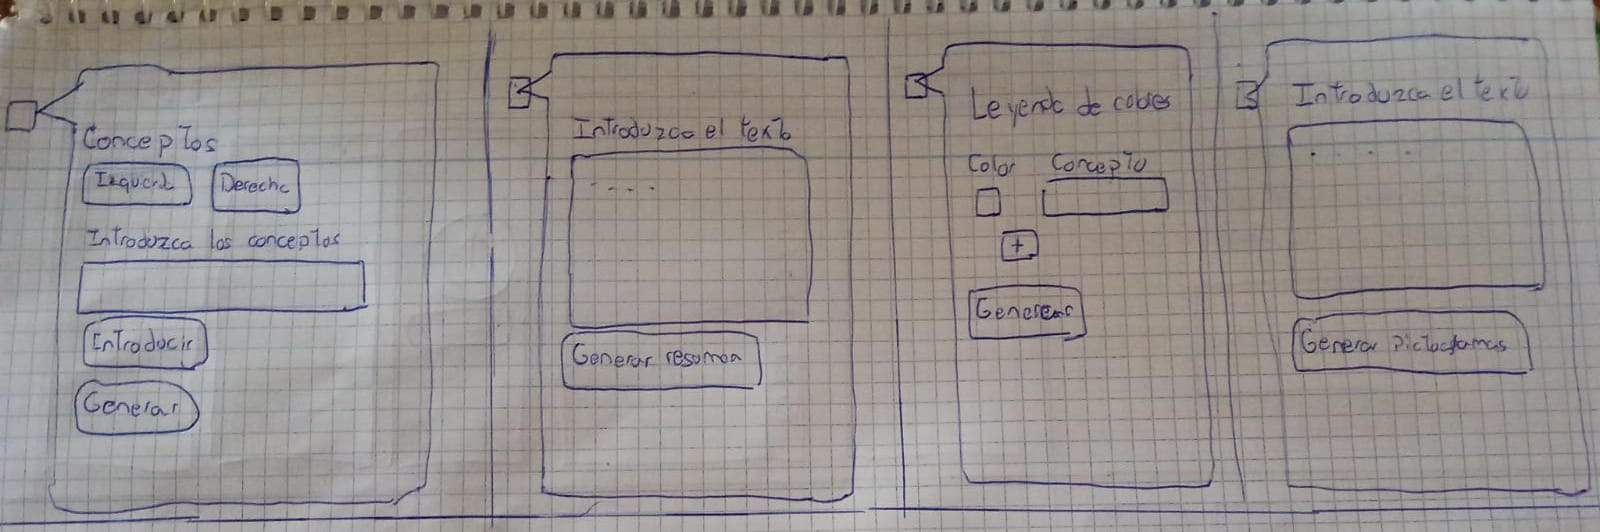
\includegraphics[width=15cm]{Diseño/Johan/Johan2.jpeg}
  \caption{Diseño de leyenda de Johan.}
  \label{Johan2}
\end{figure}

\begin{figure}[ht!]
  \centering
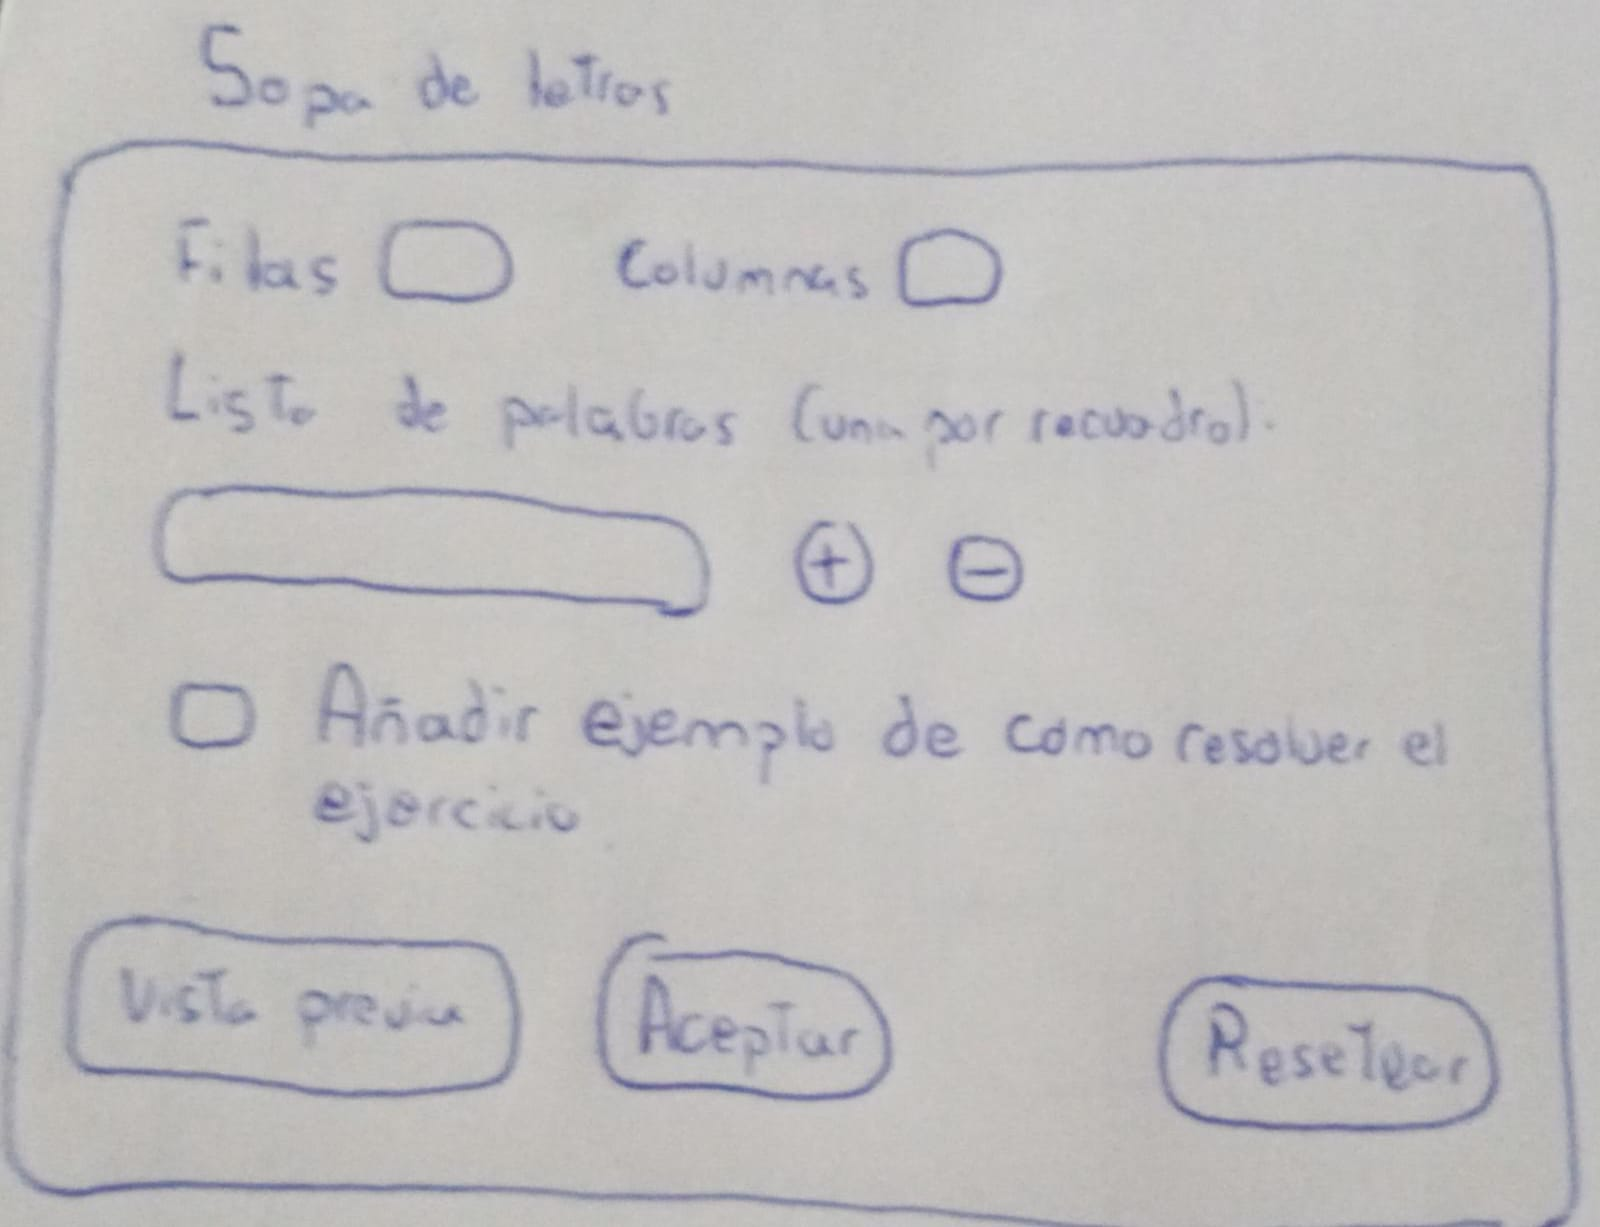
\includegraphics[width=15cm]{Diseño/Johan/Johan1.jpeg}
  \caption{Diseño de sopa de letras.}
  
  \label{Johan1}
\end{figure}






























































  
  


















































  
  